% ============================================================
%  Balancing Robot – Systemdokumentation
%  Simples, stabiles Design. Compiler: pdflatex
% ============================================================
\documentclass[11pt, a4paper]{scrreprt}

\usepackage[T1]{fontenc}
\usepackage[utf8]{inputenc}
\usepackage[ngerman]{babel}
\usepackage[a4paper, top=25mm, bottom=30mm, left=25mm, right=25mm]{geometry}
\usepackage{xcolor}
\usepackage{graphicx}
\usepackage{helvet}
\usepackage{booktabs}
\usepackage{amsmath}
\usepackage{amssymb}
\usepackage{siunitx}
\sisetup{locale = DE}
\usepackage{tikz}
\usetikzlibrary{shapes, arrows.meta, positioning}
\usepackage{enumitem}
\usepackage{pdfpages}
\usepackage{setspace}
\setstretch{1.2}
\usepackage{hyperref}

\newcommand{\posnr}[1]{(Pos.~\tikz[baseline=(c.base)]{
    \node[draw,circle,inner sep=0pt,minimum size=2ex] (c)
    {\scriptsize #1};})}

\setcounter{secnumdepth}{4}
\usepackage[automark]{scrlayer-scrpage}

\renewcommand{\familydefault}{\sfdefault}

\definecolor{htbblue}{HTML}{0078C8}

% Kopfzeile
\clearpairofpagestyles
\ohead{\pagemark}
\ihead{\headmark}
\KOMAoptions{headsepline=true}

% Überschriften blau
\addtokomafont{chapter}{\color{htbblue}}
\addtokomafont{section}{\color{htbblue}}
\addtokomafont{subsection}{\color{htbblue}}

\hypersetup{colorlinks=true, linkcolor=htbblue, urlcolor=htbblue}

% ============================================================
\begin{document}

% ── Titelseite ───────────────────────────────────────────────
\begin{titlepage}
  \vspace*{5mm}
  \IfFileExists{htw_logo.png}{%
    \hfill
\includegraphics[height=16mm]{htw_logo.png}\\[4mm]%
  }{}
  {\color{htbblue}\rule{\textwidth}{1.5pt}}
  \vspace{6mm}

  {\fontsize{32}{38}\selectfont\bfseries Balancing Robot\par}
  \vspace{4mm}
  {\Large\color{htbblue} Systemdokumentation\par}
  \vspace{6mm}
  {\color{htbblue}\rule{\textwidth}{0.5pt}}

  \vfill
  \begin{center}
    
\includegraphics[width=0.65\textwidth]{Gesamt.PNG}
  \end{center}
  \vfill

  {\normalsize
    HTW Saar – Industrielle Robotik · WiSe 2025/26\\[4pt]
    \textbf{Team:} Simon Bernarding, Marek Gerber, Sebastian Haas, Hanan Jawesh, Leon Weyand\\[4pt]
    \textbf{Datum:} \today
  }
\end{titlepage}

% ── Inhaltsverzeichnis ───────────────────────────────────────
\tableofcontents

% ============================================================
\chapter{Projektziel}

Im Rahmen der Lehrveranstaltung Industrielle Robotik an der HTW Saar (WiSe 2025/26) wurde ein ballbalancierender Roboter entwickelt. Ziel des Projekts ist es, einen Ball auf einer beweglichen Plattform mithilfe eines geschlossenen Regelkreises zu stabilisieren.

Die Plattform wird von drei Servomotoren über eine Tripod-Mechanik gekippt. Eine Kamera erfasst kontinuierlich das Bild der Plattform; eine Bildverarbeitungskomponente erkennt die aktuelle Ballposition. Ein PD-Regler berechnet daraus die notwendigen Kippwinkel der Plattform, die über die inverse Kinematik in Servowinkel umgerechnet und an die Motoren übertragen werden.

Als Recheneinheit wird ein Raspberry Pi eingesetzt, auf dem alle Komponenten (Bildverarbeitung, Regelung und Servoansteuerung) in Echtzeit ausgeführt werden.

% ============================================================
\chapter{Softwarearchitektur}

Die Software des Balancing Robots ist in mehrere voneinander unabhängige
Module aufgeteilt. Das zentrale Ziel dieser Aufteilung ist, dass jede
Komponente einzeln entwickelt, getestet und ausgetauscht werden kann,
ohne dass dabei andere Teile des Systems angepasst werden müssen.
Ein konkreter Vorteil davon ist, dass der Großteil des Codes auf einem
gewöhnlichen Laptop ausgeführt und getestet werden kann, ohne Zugriff
auf den Raspberry Pi oder die angeschlossene Hardware zu haben. Die Softwarearchitektur wurde von Leon Weyand geplant, die Implementierung erfolgte durch das gesamte Team.

\section{Modulübersicht}

Das Projekt gliedert sich in folgende Module:

\begin{center}
\begin{tabular}{ll}
  \toprule
  Modul & Aufgabe \\
  \midrule
  \texttt{balancing\_platform} & Verbindet Kinematik und Hardware, einzige Schnittstelle für den Regler \\
  \texttt{kinematik}           & Berechnet aus gewünschten Kippwinkeln die nötigen Servowinkel \\
  \texttt{hardware}            & Steuert die Servos an, enthält Pi-spezifischen Code \\
  \texttt{vision}              & Erkennt den Ball im Kamerabild und schätzt Position und Geschwindigkeit \\
  \texttt{control}             & Enthält den PD-Regler \\
  \bottomrule
\end{tabular}
\end{center}

Der Einstiegspunkt für den laufenden Betrieb ist \texttt{main\_control.py}.
Dort werden alle Komponenten instanziiert und der Regelloop gestartet.

\section{Schichtenarchitektur}

Der Regler kommuniziert ausschließlich mit der \texttt{Platform}-Klasse
aus dem Modul \texttt{balancing\_platform}. Diese Klasse ist der einzige
Berührungspunkt zwischen Regelung und dem Rest des Systems. Der Regler
muss lediglich \texttt{set\_tilt(winkel\_x, winkel\_y)} aufrufen und
bekommt keine Details darüber, wie die Winkel berechnet oder wie die
Servos angesteuert werden.

Intern ruft \texttt{Platform} für die Winkelberechnung die
\texttt{KinematicsEngine} auf und gibt die berechneten Winkel anschließend
an den \texttt{ServoDriver} weiter. \texttt{KinematicsEngine} und
\texttt{ServoDriver} haben dabei keine direkte Verbindung zueinander.

Das Modul \texttt{vision} steht dabei parallel zu \texttt{Platform} und
ist genauso entkoppelt. Es liefert dem Regler die Ballposition und
Geschwindigkeit, weiß aber nichts über Servos oder Kinematik. Der Regler
selbst ist also der einzige Punkt im System, der sowohl mit \texttt{vision}
als auch mit \texttt{Platform} kommuniziert. Abbildung~\ref{fig:komponenten}
zeigt den vollständigen Aufbau mit allen Komponenten und ihren Verbindungen.

\begin{figure}[h]
  \centering
  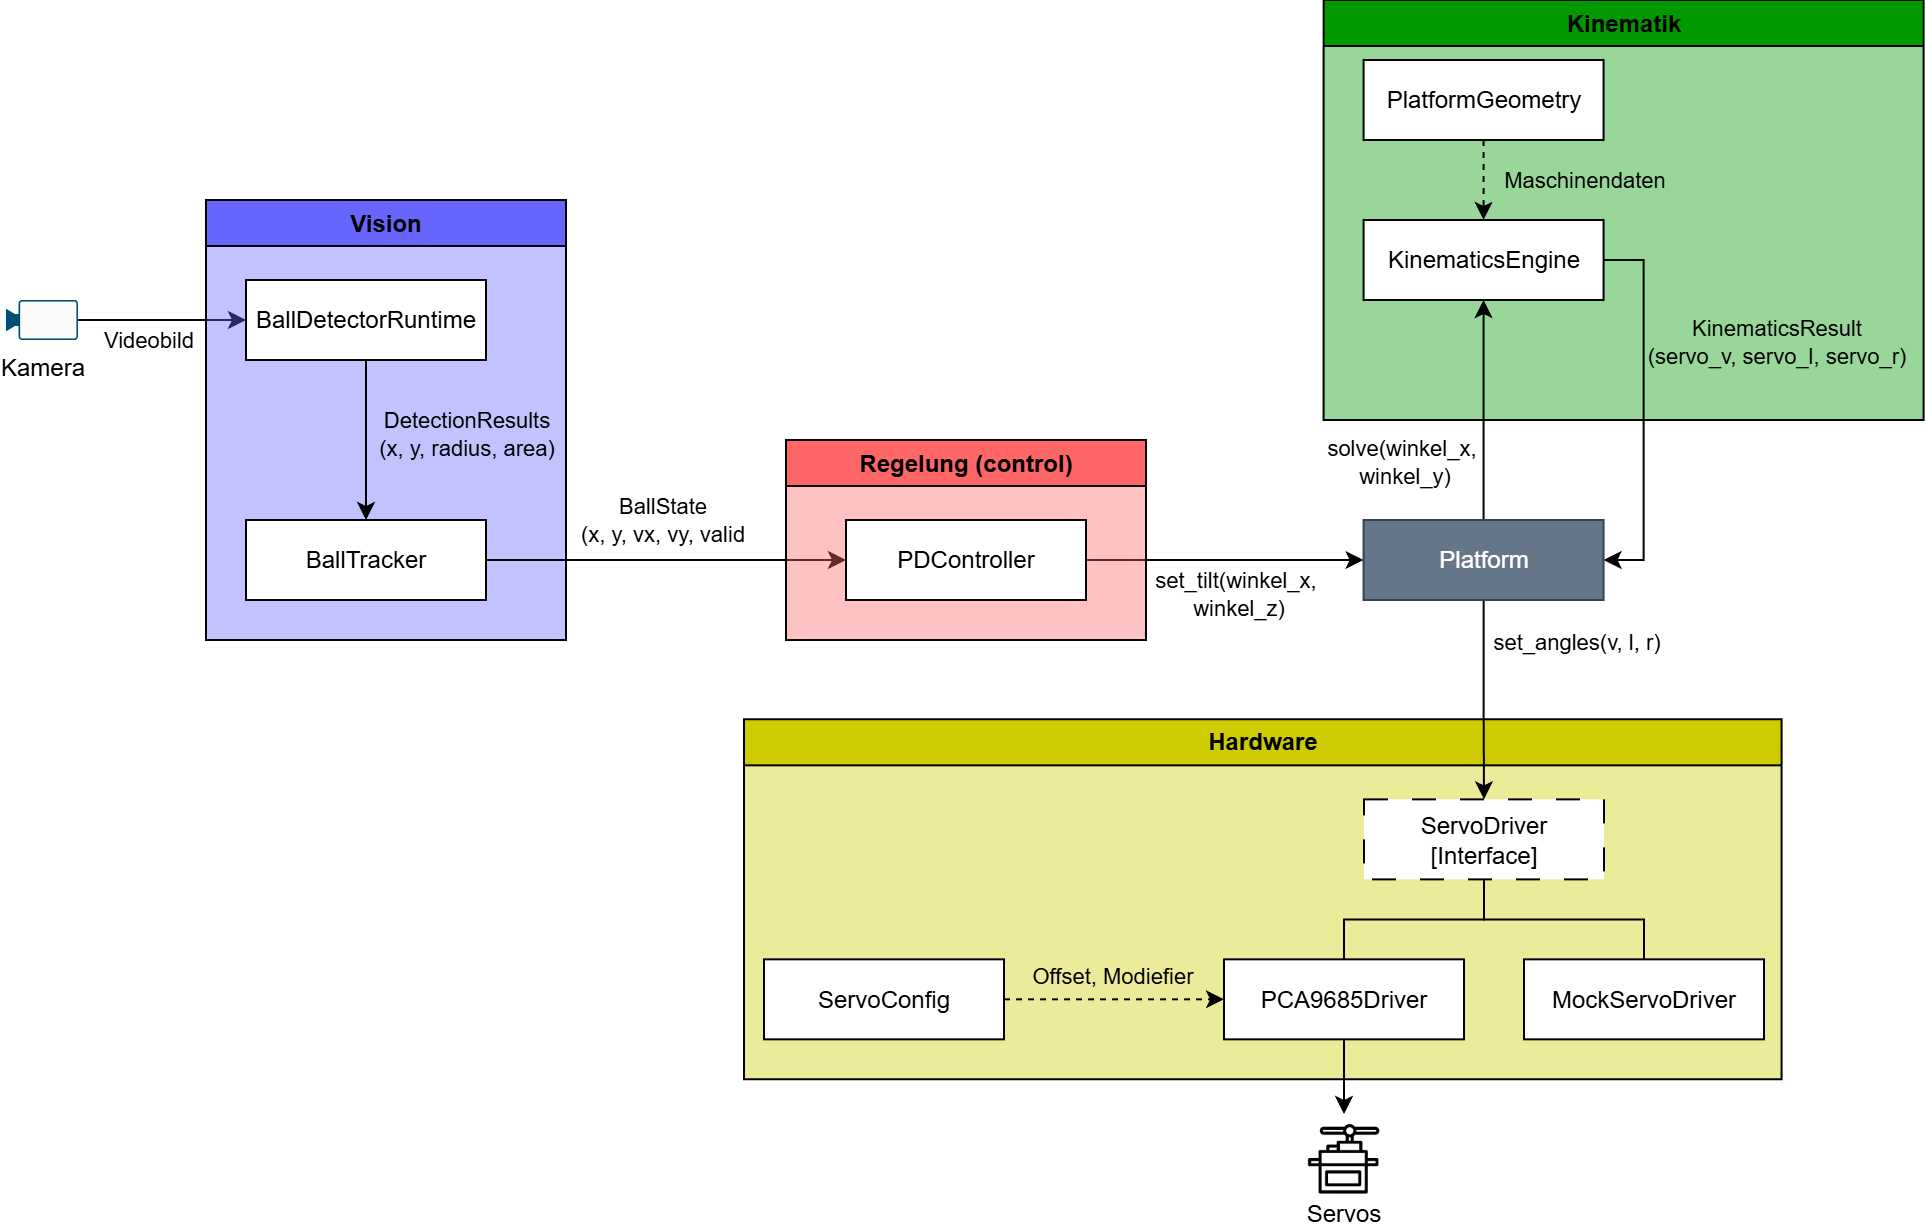
\includegraphics[width=\textwidth]{Komponenten.png}
  \caption{Komponentendiagramm der Softwarearchitektur}
  \label{fig:komponenten}
\end{figure}

Im laufenden Betrieb läuft \texttt{main\_control.py} in einer festen
Regelschleife mit 30\,Hz. Pro Durchlauf liest der Regler den aktuellen
Ballzustand aus dem \texttt{BallTracker}, berechnet die gewünschten
Kippwinkel und übergibt sie an \texttt{Platform}. Wenn kein Ball erkannt
wird, fährt die Plattform in die Neutralstellung. Die Bildverarbeitung
läuft dabei in einem eigenen Thread, sodass die Regelschleife nicht
auf ein neues Kamerabild warten muss.

\section{Hardware-Abstraktion}
\label{sec:hardware_abstraktion}

Der Pi-spezifische Code ist vollständig im Modul \texttt{hardware} gekapselt.
Alle Servo-Treiber implementieren dasselbe abstrakte Interface
\texttt{ServoDriver}, das drei Methoden vorschreibt: \texttt{set\_angles()}
setzt die drei Servos auf die angegebenen Winkel, \texttt{neutral()} fährt
alle Servos in die Ausgangsstellung, und \texttt{close()} wird beim Beenden
aufgerufen und gibt Ressourcen frei. Solange ein Treiber dieses Interface
erfüllt, kann er ohne Änderungen am restlichen Code eingesetzt werden.

Es gibt zwei konkrete Implementierungen. Der \texttt{PCA9685Driver} spricht
über den I\textsuperscript{2}C-Bus mit dem PCA9685-Servo-Controller und
wird auf dem Raspberry Pi verwendet. Er importiert \texttt{adafruit\_servokit},
eine Bibliothek die nur auf dem Pi verfügbar ist. Der \texttt{MockServoDriver}
hingegen enthält keinen Hardware-Import und gibt die berechneten Winkel
lediglich auf der Konsole aus. Er kann auf jedem Rechner ausgeführt werden.

Um das System auf dem Laptop zu testen, reicht es in \texttt{main\_control.py}
den \texttt{PCA9685Driver} durch den \texttt{MockServoDriver} zu ersetzen.
Der Rest des Codes bleibt unverändert, weil \texttt{Platform} nur gegen
das abstrakte Interface arbeitet und nicht gegen eine konkrete Implementierung.

\section{Maschinendaten und Konfiguration}

Alle geometrischen Maschinendaten des Roboters, also Plattenradius,
Schwingenlängen und Standardhöhe, sind in der Klasse \texttt{PlatformGeometry}
im Modul \texttt{kinematik} zusammengefasst. Die Klasse hat für alle
Parameter Standardwerte, die dem realen Aufbau entsprechen. So muss
beim Start nichts manuell übergeben werden, und es gibt eine einzige
Stelle im Code, an der diese Werte bei Bedarf angepasst werden.

Kalibrierungswerte, die sich je nach Aufbau oder Montage unterscheiden
können, sind davon getrennt in \texttt{ServoConfig} im Modul \texttt{hardware}
gespeichert. Dazu gehören die mechanischen Offsets der einzelnen Servos
sowie ein Multiplikator zur Invertierung der Drehrichtung. Diese Werte
können auch aus einer externen Konfigurationsdatei (\texttt{config.json})
geladen werden, sodass sie ohne Codeänderung angepasst werden können.

% ============================================================
\chapter{Mechanische Konstruktion}

Im Rahmen dieses Projektes wurde die mechanische Konstruktion und der Aufbau der Baugruppe bearbeitet. Darunter fällt die CAD-gestützte Konstruktion, die Auswahl mechanischer Komponenten, die Fertigung der Werkstücke und die Anpassung der Mechanik im Laufe des Projektes.

In der Gruppe wurde sich zunächst auf eine Platte aus Plexiglas mit dem Durchmesser \SI{250}{\milli\metre} und einer Dicke von \SI{4}{\milli\metre} geeinigt. Damit und einem zum Field of View der Kamera passenden Mindestabstand ergab sich aus der Kinematik für die Servo Kurbel \posnr{12} ein Achsabstand von \SI{70}{\milli\metre}. Für die darüberliegende Schwinge \posnr{7}\posnr{8}\posnr{9} eine Länge von \SI{179,2}{\milli\metre}.

Des Weiteren wurde ein Grunddesign gewählt, bei dem die Servokurbel in der Nulllage parallel zur Standfläche orientiert ist. Mit einem positiven und negativen Arbeitsraum ergibt sich so eine maximale Änderung der Plattform bei eher kleineren Winkeländerungen des Servowinkels. Bearbeitet wurde
dieser Teil von Simon Bernarding.

\section{Stückliste}

Die folgende Tabelle listet alle Bauteile der mechanischen Baugruppe. Der vollständige Zeichnungssatz ist in Anhang~\ref{app:zeichnungen} beigefügt.

\begin{center}
\begin{tabular}{clll}
  \toprule
  Pos. & Benennung & Anzahl & Material / Bemerkung \\
  \midrule
  1  & Grundhalter              & 1 & 3D-Druck \\
  2  & Abdeckung                & 3 & 3D-Druck \\
  3  & Innere Grundplatte       & 1 & 3D-Druck \\
  4  & Klemme Unten             & 3 & 3D-Druck \\
  5  & Klemme Oben              & 3 & 3D-Druck \\
  6  & Verspannung Lagerturm    & 3 & 3D-Druck \\
  7  & Verbinder Schwinge       & 3 & 3D-Druck \\
  8  & Schwinge Oben            & 3 & 3D-Druck \\
  9  & Schwinge Unten           & 3 & 3D-Druck \\
  10 & Lager Bolzen Knickarm    & 3 & Stahl \\
  11 & Abstandhalter Klemme     & 3 & 3D-Druck \\
  12 & Servo Kurbel             & 3 & 3D-Druck \\
  13 & Bolzen Klemme            & 3 & Stahl, M4\(\times\)0{,}7 \\
  14 & Teilstück Deckel         & 2 & 3D-Druck \\
  15 & Teilstück Deckel Schalter & 1 & 3D-Druck \\
  16 & Platte                   & 1 & Plexiglas, \(\varnothing\)\SI{250}{\milli\metre} \\
  \bottomrule
\end{tabular}
\end{center}

\section{Freiheitsgrade}
Bevor man nun das System konstruieren kann muss man die Freiheitsgrade so einschränken, dass man mit drei Servos das System zwangsgeführt beschreiben kann. Zur Berechnung ergibt sich folgende Formel

\[
F = 6(n - 1) - 6g + \sum_{i=1}^{g} f_i
\]

Hierbei bezeichnet \(n\) die Anzahl der starren Körper einschließlich des Gestells, \(g\) die Anzahl der Gelenke und \(f_i\) den Freiheitsgrad des jeweiligen Gelenks.

Der Tripod besteht aus einem Grundkörper, einer beweglichen Plattform und drei identischen Knickarmen. Baut man einen Knickarm als \(\mathrm{R\!-\!R\!-\!S}\)-Kette auf, was bedeutet ein unteres \textbf{R}otationsgelenk am Motor, ein weiteres \textbf{R}otationsgelenk am Knickarm sowie ein oberes \textbf{S}phärisches Gelenk an der Plattform. Damit ergibt sich pro Bein eine Summe von \(1+1+3=5\) Gelenkfreiheitsgraden.
\newpage

Für drei Beine folgt somit:

\[
\sum_{i=1}^{g} f_i = 3 \cdot 5 = 15
\]

Die Anzahl der starren Körper beträgt insgesamt \(n=8\), bestehend aus dem Gestell, der beweglichen Plattform und je zwei beweglichen Gliedern pro Bein. Die Anzahl der Gelenke beträgt insgesamt \(g=9\), da jedes der drei Beine aus drei Gelenken besteht.

Durch Einsetzen in die Formel ergibt sich:

\[
F = 6(8 - 1) - 6 \cdot 9 + 15 = 42 - 54 + 15 = 3
\]

Der Tripod besitzt somit drei Freiheitsgrade, und ist so mit drei Motoren zwangsgeführt.




\section{Konstruieren der Ersten Version}
Nachdem die Grundvoraussetzungen definiert worden waren, wurde eine erste Baugruppe abgeleitet und gefertigt. Dieses Modell ist in Abbildung~\ref{fig:V1_Zusammenbau} dargestellt. Nach dem Zusammenbau wurden jedoch Schwachstellen in der Konstruktion deutlich, welche im Laufe dieses Abschnitts erläutert werden.

\begin{figure}[h!]
	\centering
	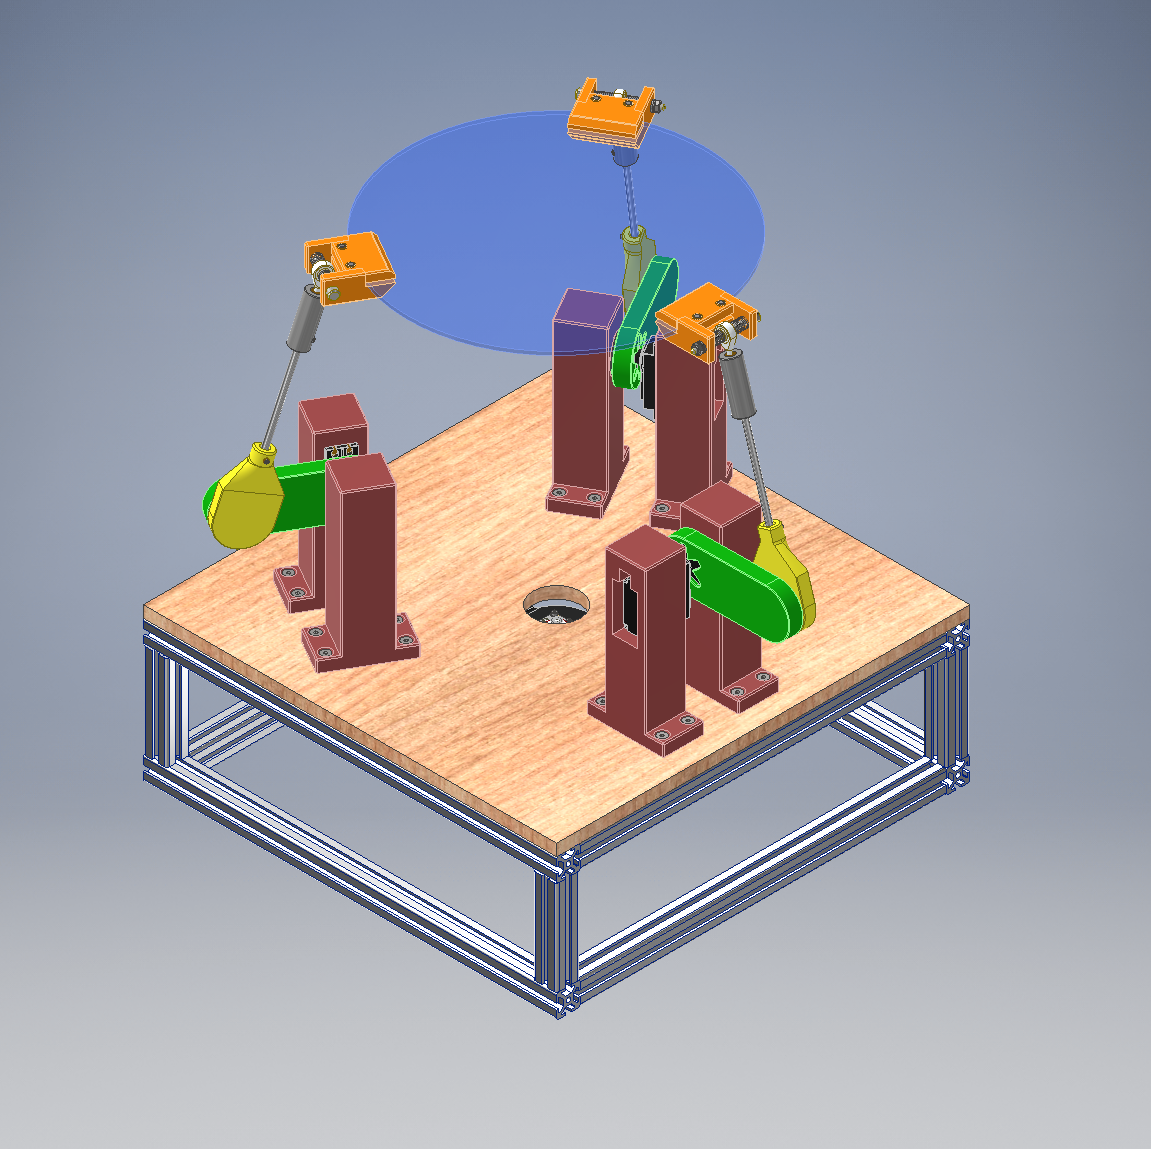
\includegraphics[width=0.4\textwidth]{Abbildungen/Zusammenbau_Version1.png}
	\caption[Zusammenbau der ersten Projektversion]{Zusammenbau der ersten Projektversion}
	\label{fig:V1_Zusammenbau}
\end{figure}

Zum einen war, wie in Abbildung~\ref{fig:V1_ArmLager} dargestellt, das mittlere Gelenk des Knickarms als Kugellager ausgeführt, in welches ein Zapfen eingepresst wurde. Dabei wurden jedoch zwei Probleme ersichtlich. Zum einen wirkte sich das Lagerspiel vollständig aus und wurde nicht abgefangen. Dies hatte zur Folge, dass die Plattform bei Bewegungen merklich schwankte. Zum anderen entstanden dadurch Querkräfte auf dem Bolzen im Innenring des Lagers, wodurch dieser an der Kante des Innenrings als Schwachstelle abbrach.

\begin{figure}[h!]
	\centering
	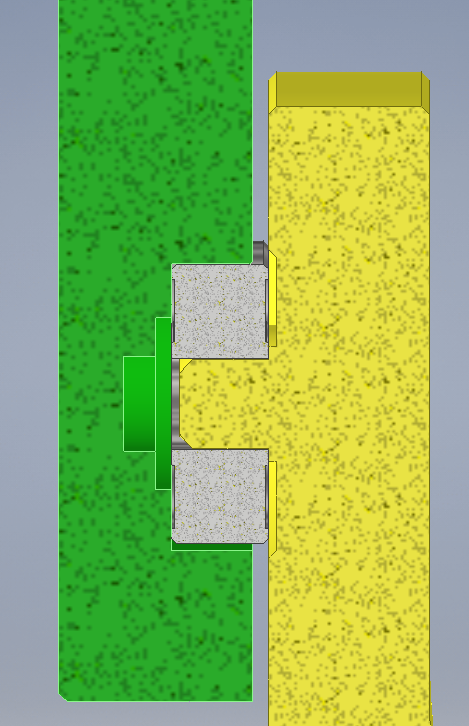
\includegraphics[width=0.2\textwidth]{Abbildungen/V1_ArmLager.PNG}
	\caption[Mittleres Knickarmgelenk im Schnitt]{Mittleres Knickarmgelenk im Schnitt}
	\label{fig:V1_ArmLager}
\end{figure}

Zusätzlich zu den konstruktiven Problemen wurde schnell deutlich, dass eine eckige Grundplatte nicht zu einer runden Anordnung der Knickarme passt.

Dennoch wurde diese Version fertiggestellt. Ein Abbrechen der Lagerbolzen konnte durch eine veränderte Orientierung des Bauteils während des 3D-Drucks verhindert werden. Dadurch konnten die anderen Teilbereiche des Projekts bereits mit diesem System arbeiten sowie ihre eigenen Entwicklungen testen und verbessern.



\section{Verbesserung der Mechanik mit zweiter Version}
Um die Fehler der ersten Version zu beheben, wurde diese vollständig überarbeitet. Ziel dieser Neugestaltung war es, zum einen die Ungenauigkeit infolge des vorhandenen Lagerspiels zu verringern, die Lagerverbindungen zu verstärken, eine optisch ansprechendere Designwahl zu treffen und das System stärker einzuhausen, um einen homogeneren Gesamtaufbau zu erzielen. Die gesamte Baugruppe ist in Abbildung~\ref{fig:GesamtV2} dargestellt.

\begin{figure}[h!]
	\centering
	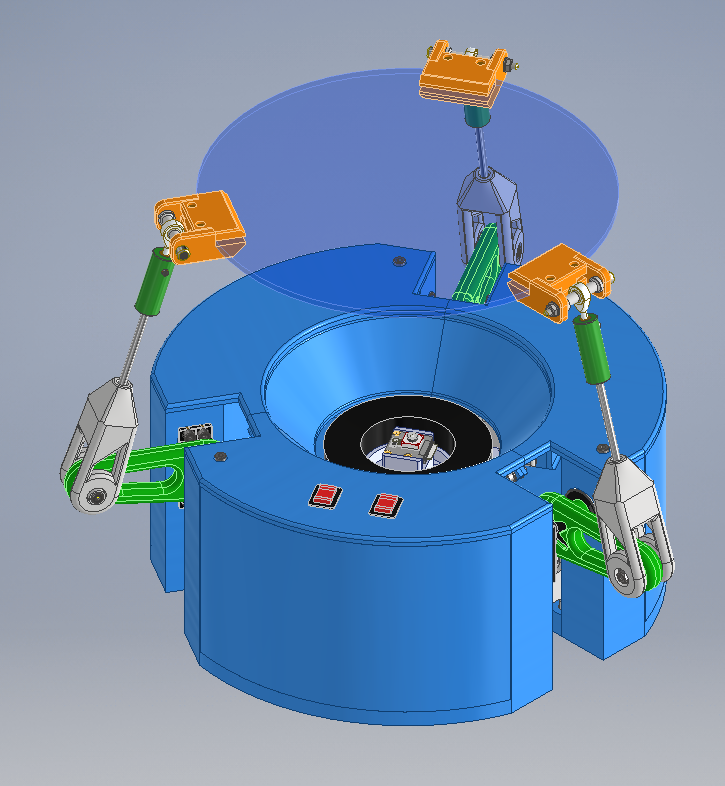
\includegraphics[width=0.3\textwidth]{Abbildungen/Gesamt.PNG}
	\caption[Gesamtaufbau der zweiten Version]{Gesamtaufbau der zweiten Version}
	\label{fig:GesamtV2}
\end{figure}

\newpage
\subsection{Lagersitz}
In Abbildung~\ref{fig:Lagersitz} ist beispielhaft der Lagersitz des Außenrings im Knickgelenk dargestellt. Jeder Lagersitz ist prinzipiell gleich aufgebaut. Der größere äußere Ring ist im Durchmesser um \SI{2}{\milli\metre} größer als der Außendurchmesser des Rillenkugellagers. Die davon ausgehenden Vorsprünge besitzen den Außendurchmesser des Lagers. Dadurch kann dieses in den Sitz eingepresst werden. Diese Lösung wurde gewählt, da das Lager so auch dann zentriert und sauber in Position sitzt, wenn der 3D-Drucker aufgrund seiner Fertigungstoleranzen keinen perfekt kreisförmigen Sitz druckt. Die Vorsprünge sind in ungerader Anzahl kreisförmig angeordnet. Dadurch wird verhindert, dass sich zwei Vorsprünge direkt gegenüberstehen. Im hinteren Teil des Lagersitzes ist die Fläche durch eine Bohrung ausgespart, damit der Innenring bei Bewegung nicht am Material reibt.

\begin{figure}[h!]
	\centering
	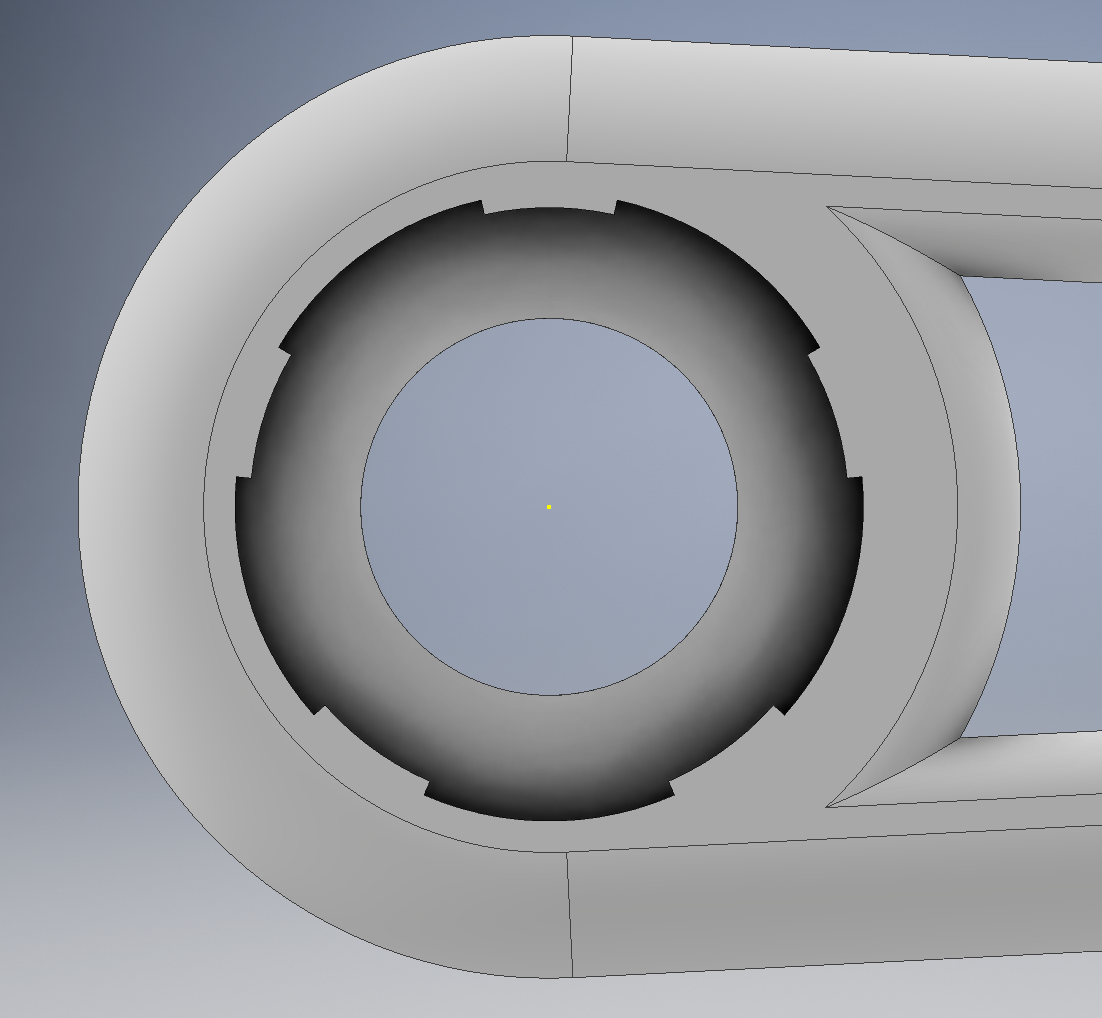
\includegraphics[width=0.4\textwidth]{Abbildungen/Lagersitz.PNG}
	\caption[Lagersitz Knickarm]{Lagersitz Knickarm}
	\label{fig:Lagersitz}
\end{figure}

\newpage

\subsection{Neue Lagerung Mittleres Knickarmgelenk}
Die in Abbildung~\ref{fig:Knickarmlagerung} gezeigte neue Variante des mittleren Knickarmgelenks wurde gegenüber der Vorgängerversion grundlegend überarbeitet. Im Gegensatz zur ersten Ausführung ist das Gelenk nun symmetrisch durch ein umgreifendes Bauteil der unteren Schwinge \posnr{9} ausgeführt. In diesem Bauteil sitzen zwei Rillenkugellager, die über ihre Innenringe mittels einer Passhülse und einer Schraubverbindung auf der Servokurbel \posnr{12} geklemmt sind. Dadurch konnte das zuvor zu große Lagerspiel deutlich reduziert werden, sodass es die Bewegung beim Verfahren der Motoren nicht mehr merklich beeinträchtigt.

\begin{figure}[h!]
	\centering
	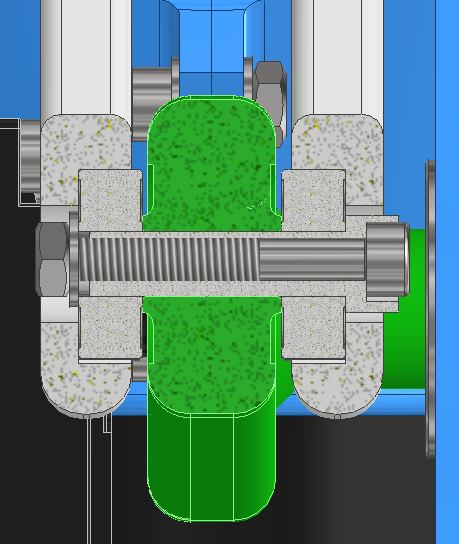
\includegraphics[width=0.3\textwidth]{Abbildungen/LagersitzKnickarmNeu.PNG}
	\caption[Neue Lagerung mittleres Knickarmgelenk]{Neue Lagerung mittleres Knickarmgelenk}
	\label{fig:Knickarmlagerung}
\end{figure}



\subsection{Weitere Merkmale der Konstruktion}
Die Konstruktion musste aufgrund der begrenzten Bauraumgröße des 3D-Druckers in drei Teile aufgeteilt werden. Diese Teile werden zum einen über die Lagerungen der Knickarme miteinander verbunden, zum anderen jedoch auch im Inneren der Lagertürme des Grundhalters \posnr{1} jeweils mit dem Bauteil \textit{Verspannung Lagerturm} \posnr{6} ausgesteift. In der Mitte der Baugruppe wird zu demselben Zweck die innere Grundplatte \posnr{3} verschraubt. Dadurch werden mögliche von außen einwirkende Kräfte und Momente nicht über die Lager abgeleitet, sodass der Knickarm unbeeinflusst bleibt. Diese Versteifungen sind so ausgeführt, dass gegebenenfalls Toleranzen der drei Einzelteile ausgeglichen werden können. Zusätzlich sind die Teile des Deckels untereinander sowie mit der Konstruktion verschraubt, was die Stabilität nach oben hin weiter erhöht.

% ============================================================
\chapter{Elektronik \& Gehäuse}

Im Rahmen des Projekts wurde der Bereich Entwicklung und Umsetzung der elektronischen
Infrastruktur bearbeitet. Dies umfasste insbesondere die Planung und Realisierung der
Spannungsversorgung, das Verschalten der einzelnen Komponenten sowie die Konzeption und
Fertigung eines passenden Gehäuses für den gesamten Technik-Stack. Zusätzlich wurden
spezifische Halterungen für den Mikrocontroller und die Kamera entwickelt und integriert.
Ziel war es, ein zuverlässiges, sicheres und übersichtliches System zu schaffen, das sowohl
funktional als auch mechanisch stabil ist. Bearbeitet wurde dieser Teil von Marek Gerber.

\section{Anforderungen und Planung}

Zu Beginn wurden die Anforderungen an die Elektronik und Mechanik definiert:

\begin{itemize}
  \item Gemeinsame Versorgung aller Komponenten mit geeigneter Spannung und Stromstärke
  \item Übersichtliche und wartungsfreundliche Verkabelung
  \item Mechanisch stabiles und kompaktes Gehäuse
  \item Sichere Befestigung von Mikrocontroller und Kamera; die Höhe der Kamera sollte noch modifizierbar sein
  \item Montagefreundlichkeit, gute Zugänglichkeit für Wartung und Erweiterungen
\end{itemize}

\section{Spannungsversorgung}

Die Spannungsversorgung wurde zentral ausgelegt und bildet die Grundlage für den stabilen
Betrieb des Systems.

Umsetzung:

\begin{itemize}
  \item Einsatz eines zentralen 24\,V Netzteils, das als externes Netzteil umgesetzt wurde,
        sodass im Projektgehäuse nur mit Spannungen im Schutzkleinspannungsbereich gearbeitet
        werden musste.
  \item Verwendung von Spannungsreglern. Es wurde ein Step-Down-Wandler verwendet, um die
        Spannungsversorgung auf 5\,V Niveau für den MC und die Servos bereitzustellen.
  \item Das optional zuschaltbare Ringlicht wurde direkt an die 24\,V Spannungsversorgung
        angebunden. Um das Licht optional zuschalten zu können, wurde ein Schalter vorgesehen.
\end{itemize}

\subsection{Verwendete Komponenten}

\begin{center}
\begin{tabular}{llllr}
  \toprule
  Pos & Bez. & Typ & Anzahl & Stückpreis \\
  \midrule
  1 & Netzteil    & Taormey-2406        & 1 & 15{,}99\,€ \\
  2 & Step-Down   & AZCelivery XL4016   & 1 & 10{,}99\,€ \\
  3 & PWM Driver  & SunFouner PCA9685   & 1 & 13{,}99\,€ \\
  \bottomrule
\end{tabular}
\end{center}

\subsection{Schaltnetzteil}

Als Netzteil wurde ein kostengünstiges Universalnetzteil eingesetzt, das bei 24\,V Spannung
einen Maximalstrom von 6\,A liefern kann. Der AC-seitige Anschluss erfolgt über einen
Kaltgerätestecker. Auf der Niederspannungs-DC-Seite wird ein 6{,}3\,mm Rundstecker verwendet.

\subsection{Step-Down-Regler}

Um die Spannungsebene zur Versorgung der Servos und des MC herzustellen, wurde ein
Step-Down-Regler verwendet. Dieser stellt bei einem Eingangsspannungsbereich von 5--40\,V
eine Ausgangsspannung von 1{,}2 bis 35\,V bereit. Der Regler hat eine Leistung von maximal
140\,W. Bei der Auswahl wurde auf eine gute Spannungsstabilisierung mit großer
Kondensator-Kapazität geachtet, damit die Leistungsspitzen beim Verfahren der Servos gut
abgepuffert werden können.

\subsection{Servo-Driver}

Erste Versuche mit dem Aufbau zeigten, dass die Software-PWM-Ausgänge am Raspberry Pi nicht
geeignet für die angestrebte Verwendung waren. Deshalb wurde ein externer PWM-Driver verwendet. Dieser kann bis zu 16 Kanäle mit Hardware-PWM bereitstellen.

\section{Gehäuseentwicklung}

Das Gehäuse wurde als tragende Struktur für alle Komponenten konzipiert.

Umsetzung:

\begin{itemize}
  \item Konstruktion mittels CAD, um anschließend die Fertigung im 3D-Druckverfahren zu ermöglichen.
  \item Integration von Befestigungspunkten für alle Bauteile, in die M2{,}5-Einschmelzmuttern
        eingesetzt werden.
  \item Kabeldurchführungen und Belüftungsöffnungen.
\end{itemize}

\begin{figure}[h]
  \centering
  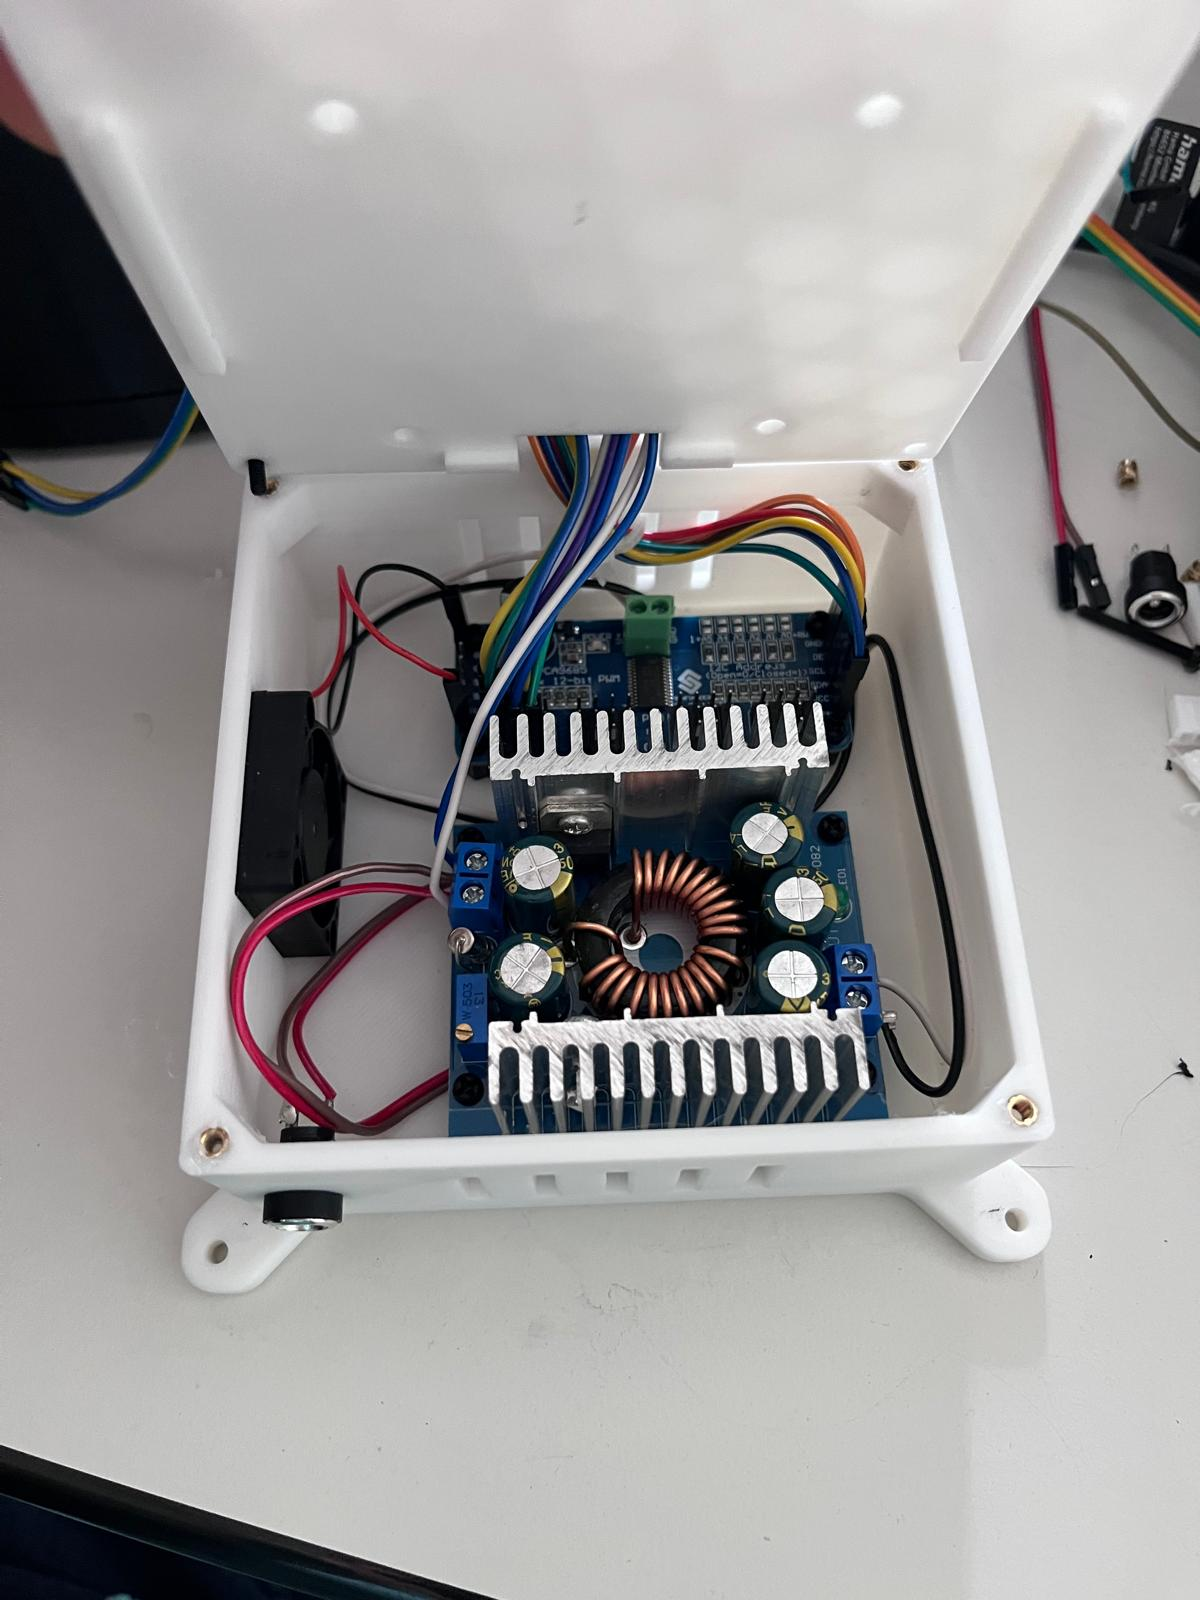
\includegraphics[width=0.6\textwidth]{E1.jpg}
  \caption{Technikbox im Gehäuse, geöffnet}
\end{figure}

\begin{figure}[h]
  \centering
  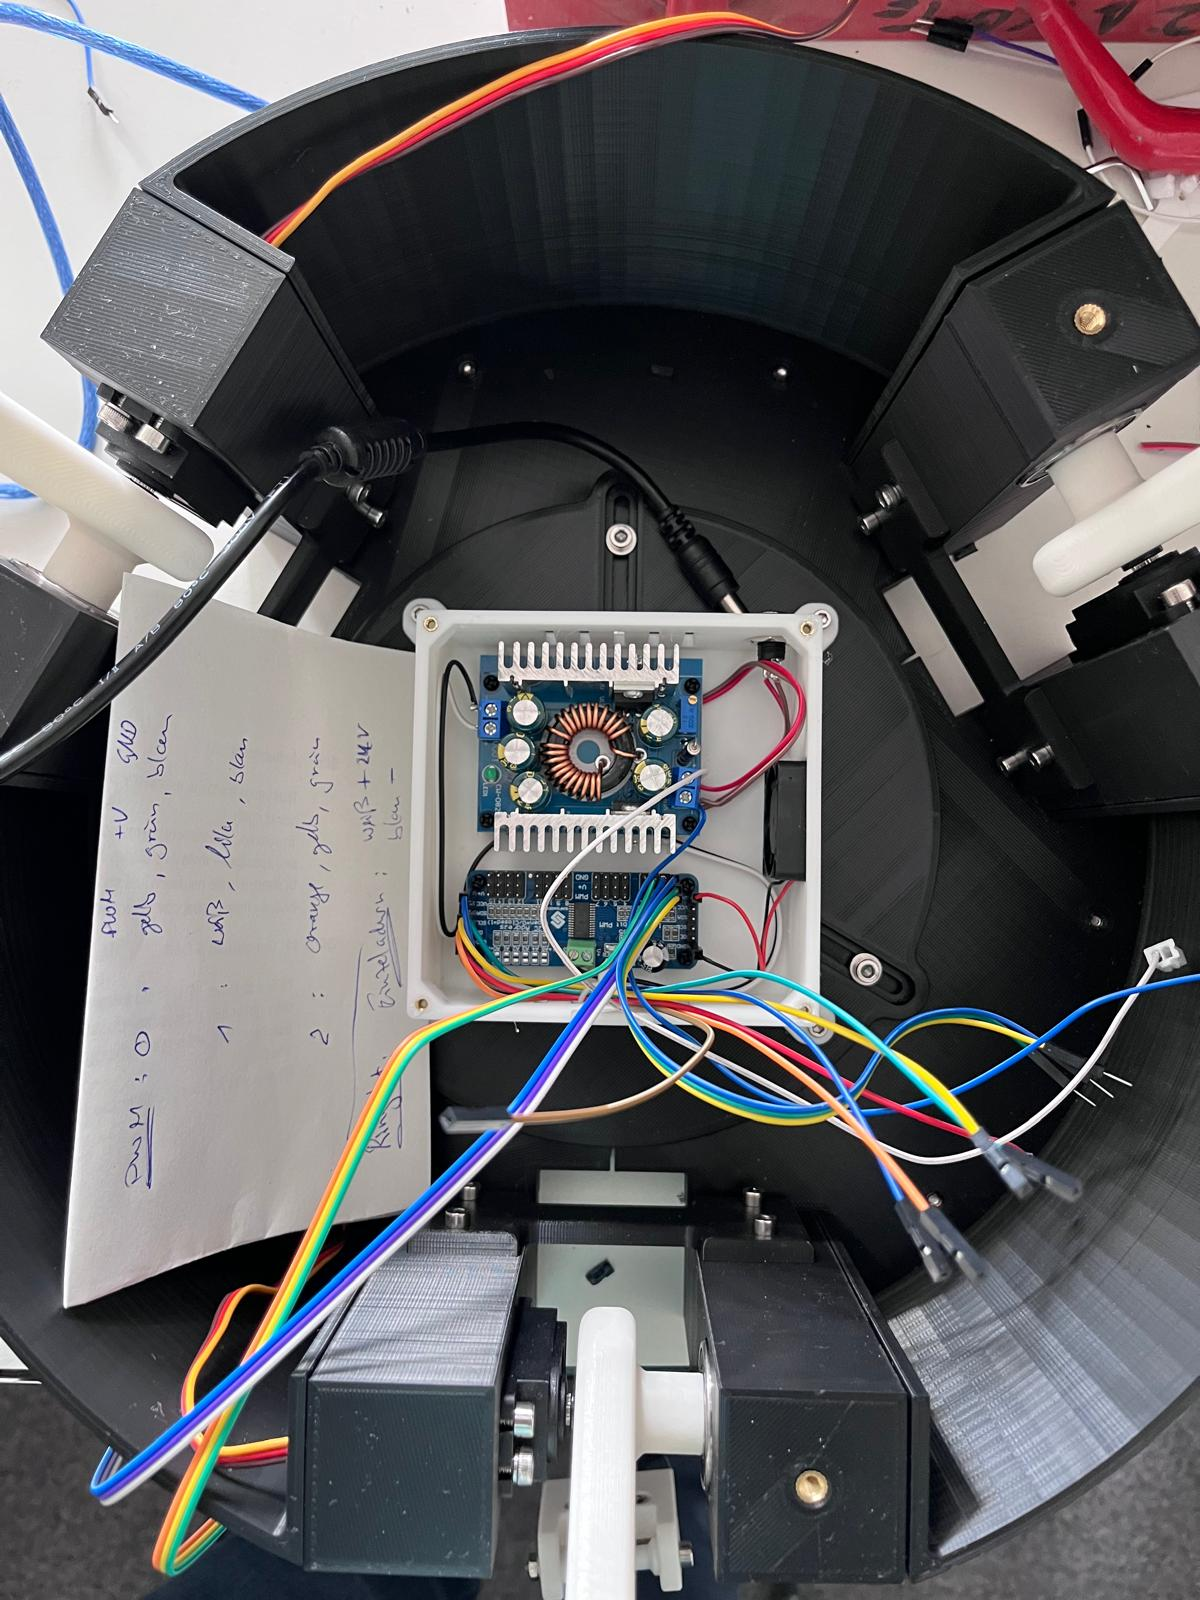
\includegraphics[width=0.6\textwidth]{E3.jpg}
  \caption{Verkabelung der Technikbox im eingebauten Zustand}
\end{figure}

% ============================================================
\chapter{Kinematik}

Das Ziel der Kinematik ist die Plattform im Raum um vorgegebene Winkel um die X- und Y-Achse
drehen zu können, sowie ihre Höhe einzustellen. Dafür stehen 3 Servos mit 3 Armen zur
Verfügung, die in 120° Schritten an der Plattform befestigt sind. Diese Arme können sich nur vor,
zurück und hoch, bzw. runter bewegen. Ein Verkippen ist nicht möglich.

Um die Plattform in die gewünschte Pose einstellen zu können, müssen die Servos verfahren
werden. Die Rückwärtskinematik dient dazu zu berechnen, welche Einstellwinkel dort benötigt
werden. Dafür wird zunächst die Plattform um die gewünschten Winkel gedreht, in der Höhe
verschoben und anschließend kontrolliert, ob die Position erreichbar ist. Danach wird für jeden
Arm der benötigte Stellwinkel des Servos ausgerechnet.

Dieses Vorgehen wird in den folgenden Unterkapiteln genauer beschrieben. Bearbeitet wurde
dieser Teil von Sebastian Haas.

\section{Drehen der Plattform}

Der erste Schritt der Rückwärtskinematik ist es, die Plattform im Raum zu platzieren, da dadurch
dann auch bekannt wird, wo die einzelnen Koppelpunkte zu den Armen liegen, wodurch sich dann
Rückschlüsse zu den Stellwinkeln der Servos ziehen lassen.

Zunächst lässt sich jeder Punkt auf der Plattform als Teil einer Ebene beschreiben. Diese Ebene
lässt sich durch einen Normalenvektor und eine Konstante d beschreiben. Für jeden Punkt auf der
Plattform muss dann folgende Gleichung gelten:

\[
  0 = n_x \cdot x + n_y \cdot y + n_z \cdot z + d
\]

Für eine waagerechte Plattform, in der X-Y-Ebene würde der Normalenvektor $n$ wie folgt aussehen:

\[
  n = \begin{pmatrix} n_x \\ n_y \\ n_z \end{pmatrix} = \begin{pmatrix} 0 \\ 0 \\ 1 \end{pmatrix}
\]

Soll die Plattform und damit die Ebene um die X-Achse mit dem Winkel $\alpha$ und um die Y-Achse mit
dem Winkel $\varphi$ gedreht werden, so kann einfach der Normalenvektor $n$ der ebenen Position mit zwei
Rotationsmatrizen gedreht werden:

\[
  n =
  \begin{pmatrix} 1 & 0 & 0 \\ 0 & \cos\alpha & -\sin\alpha \\ 0 & \sin\alpha & \cos\alpha \end{pmatrix}
  \cdot
  \begin{pmatrix} \cos\varphi & 0 & \sin\varphi \\ 0 & 1 & 0 \\ -\sin\varphi & 0 & \cos\varphi \end{pmatrix}
  \cdot
  \begin{pmatrix} 0 \\ 0 \\ 1 \end{pmatrix}
\]

Dieser neue Normalenvektor $n$ kann in die Ebenengleichung eingesetzt werden. Um die Konstante
$d$ zu erhalten, muss ein Punkt $P(x, y, z)$, der Teil der Ebene sein soll, in die Gleichung eingesetzt
werden und diese nach $d$ aufgelöst werden.

Da alle Punkte auf der Plattform in dieser Ebene liegen, liegen auch die Endpunkte der Arme in
dieser gedrehten Ebene. Gleichzeitig müssen die Endpunkte der Arme aber auch innerhalb des
jeweiligen Bewegungsraums der Arme befinden, welcher zunächst als Ebene orthogonal zur
Servowelle angenommen werden kann. Die möglichen Positionen für die Endpunkte liegen also
jeweils auf der Schnittgeraden beider Ebenen. Diese Gerade kann man sich vorstellen, als die
Gerade zwischen der Ordinate und dem Endpunkt der Servowelle, die zwar eigentlich Eben wäre,
aber stattdessen um eine Z-Steigung $a_z$ ergänzt wurde, sodass sie in der gedrehten Plattform-Ebene liegt.

Für den vorderen Arm, der sich in der Y-Z-Ebene bewegt (also immer $x = 0$), würde diese Gerade
wie folgt aussehen:

\[
  g_v(t_v) = \begin{pmatrix} 0 \\ 0 \\ 0 \end{pmatrix} + t_v \cdot \begin{pmatrix} 0 \\ 1 \\ a_v \end{pmatrix}
\]

Die Steigung $a_v$ ist dabei abhängig von der Ausrichtung der Plattform. Hier kann sich zur Hilfe
genommen werden, dass alle Vektoren und Strecken innerhalb einer Ebene, also auch diese
Gerade, rechtwinklig zum Normalenvektor sind. Sind zwei Vektoren rechtwinklig, so ist ihr
Skalarprodukt gleich Null. Also muss folgende Gleichung gelten:

\[
  0 = 0 \cdot n_x + 1 \cdot n_y + a_v \cdot n_z
\]

Mit dieser Gleichung lässt sich $a_v$ berechnen und somit alle möglichen Endpunkte des vorderen
Arms für diese Plattformlage beschreiben. Das Gleiche Vorgehen ist für die anderen beiden
Endpunkte möglich:

\[
  g_l(t_l) = \begin{pmatrix} 0 \\ 0 \\ 0 \end{pmatrix} + t_l \cdot \begin{pmatrix} -1 \\ -\tan(30°) \\ a_l \end{pmatrix}
  \qquad
  g_r(t_r) = \begin{pmatrix} 0 \\ 0 \\ 0 \end{pmatrix} + t_r \cdot \begin{pmatrix} 1 \\ -\tan(30°) \\ a_r \end{pmatrix}
\]

Somit lassen sich alle möglichen Endpunkte für eine jeweilige Plattformorientierung berechnen.
Allerdings müssen die Endpunkte der Arme noch weitere Bedingungen erfüllen. Denn diese sind
fest auf der Plattform in 120° Schritten montiert und da die Plattform starr ist, ändert sich das
Verhältnis zwischen ihnen auch nicht. Sie haben alle denselben Abstand zueinander
(„Außenlänge") und jeweils denselben Abstand („Radius") zum Mittelpunkt.

Werden nun drei Punkte gesucht, die auf jeweils einer der drei Geraden liegen und alle
Untereinander den selben Abstand zueinander haben, nämlich die Außenlänge, ergeben sich
folgende drei Gleichungen:

\begin{align*}
  \text{Außenlänge} &= \sqrt{(t_v \cdot 0 - t_l \cdot (-1))^2 + (t_v \cdot 1 - t_l \cdot (-\tan(30°)))^2 + (t_v \cdot a_v - t_l \cdot a_l)^2} \\[4pt]
  \text{Außenlänge} &= \sqrt{(t_v \cdot 0 - t_r \cdot 1)^2 + (t_v \cdot 1 - t_r \cdot (-\tan(30°)))^2 + (t_v \cdot a_v - t_r \cdot a_l)^2} \\[4pt]
  \text{Außenlänge} &= \sqrt{(t_l \cdot (-1) - t_r \cdot 1)^2 + (t_l \cdot (-\tan(30°)) - t_r \cdot (-\tan(30°)))^2 + (t_l \cdot a_l - t_r \cdot a_l)^2}
\end{align*}

Diese drei Gleichungen haben drei Unbekannte, namentlich die Längen der Schnittgeraden. Wird
dieses Gleichungssystem zum Beispiel unter Zuhilfenahme numerischer Methoden gelöst, lassen
sich so also mögliche Endpunkte für eine Pose berechnen. Dabei ist es möglich, dass sich die
Plattform in X- und Y-Richtung verschiebt, sowie um die Z-Achse verdreht.

Anschließend können alle Punkte noch gleichmäßig in der Z-Höhe verschoben, um die Plattform
auf die richtige Höhe zu bringen.

In der Software wird dies mit der Funktion \texttt{func\_kinematik\_main} umgesetzt (Ablauf
vgl.\,Abbildung~\ref{fig:ablauf_kinematik}). Dieser werden Systemparameter, sowie die gewünschten Winkel und der auf
konstanter Höhe zu haltende Punkt übergeben. Innerhalb dieser Funktion wird dann zunächst wie
oben beschrieben ein gedrehter Normalenvektor berechnet und die Schnittgeraden zu dem
Bewegungsraum der Armen aufgestellt. Anschließend wird ein Solver verwendet, um die Punkte
mit den gleichen Abständen zu finden. Bei diesem Vorgehen wird bis dahin angenommen, dass
die Plattform in Z-Richtung auf der Höhe Null liegt. Um jedoch die Höhe des Referenzpunktes
konstant zu halten, wird mit dem Normalenvektor und diesem Punkt die Konstante $d$ für die
Ebenengleichung berechnet. Mit der Ebenengleichung und den X/Y-Koordinaten der Endpunkte
lässt sich deren neue Höhe berechnen.

Nachfolgend muss dann geprüft werden, ob diese Ausrichtung der Plattform erreichbar ist. Dies
wird im Detail im folgenden Kapitel erklärt. In der Funktion \texttt{func\_kinematik\_main} werden dann
die Ergebnisse ausgewertet. Sollte die Position erreichbar sein, selbst wenn dies Anpassungen
der Höhe bedarf, wird zum nächsten Schritt übergegangen und eventuell Anpassungen
vorgenommen. Sollte die Drehung in keiner Höhe erreichbar sein, werden beide Winkel auf 95\,\%
reduziert und die vorherigen Berechnungen werden wiederholt.

Wenn eine erreichbare Position gefunden wurde, werden die benötigten Stellwinkel der Servos
berechnet. Die dafür verwendete Funktion wird im Kapitel „Errechnen der Servo-Stellwinkel"
näher beschrieben.

Am Ende der Funktion werden alle Servo-Stellwinkel, sowie die Parameter der aktuellen
Ebenengleichung die eventuell angepassten Winkel zurück übergeben.

\begin{figure}[h]
  \centering
  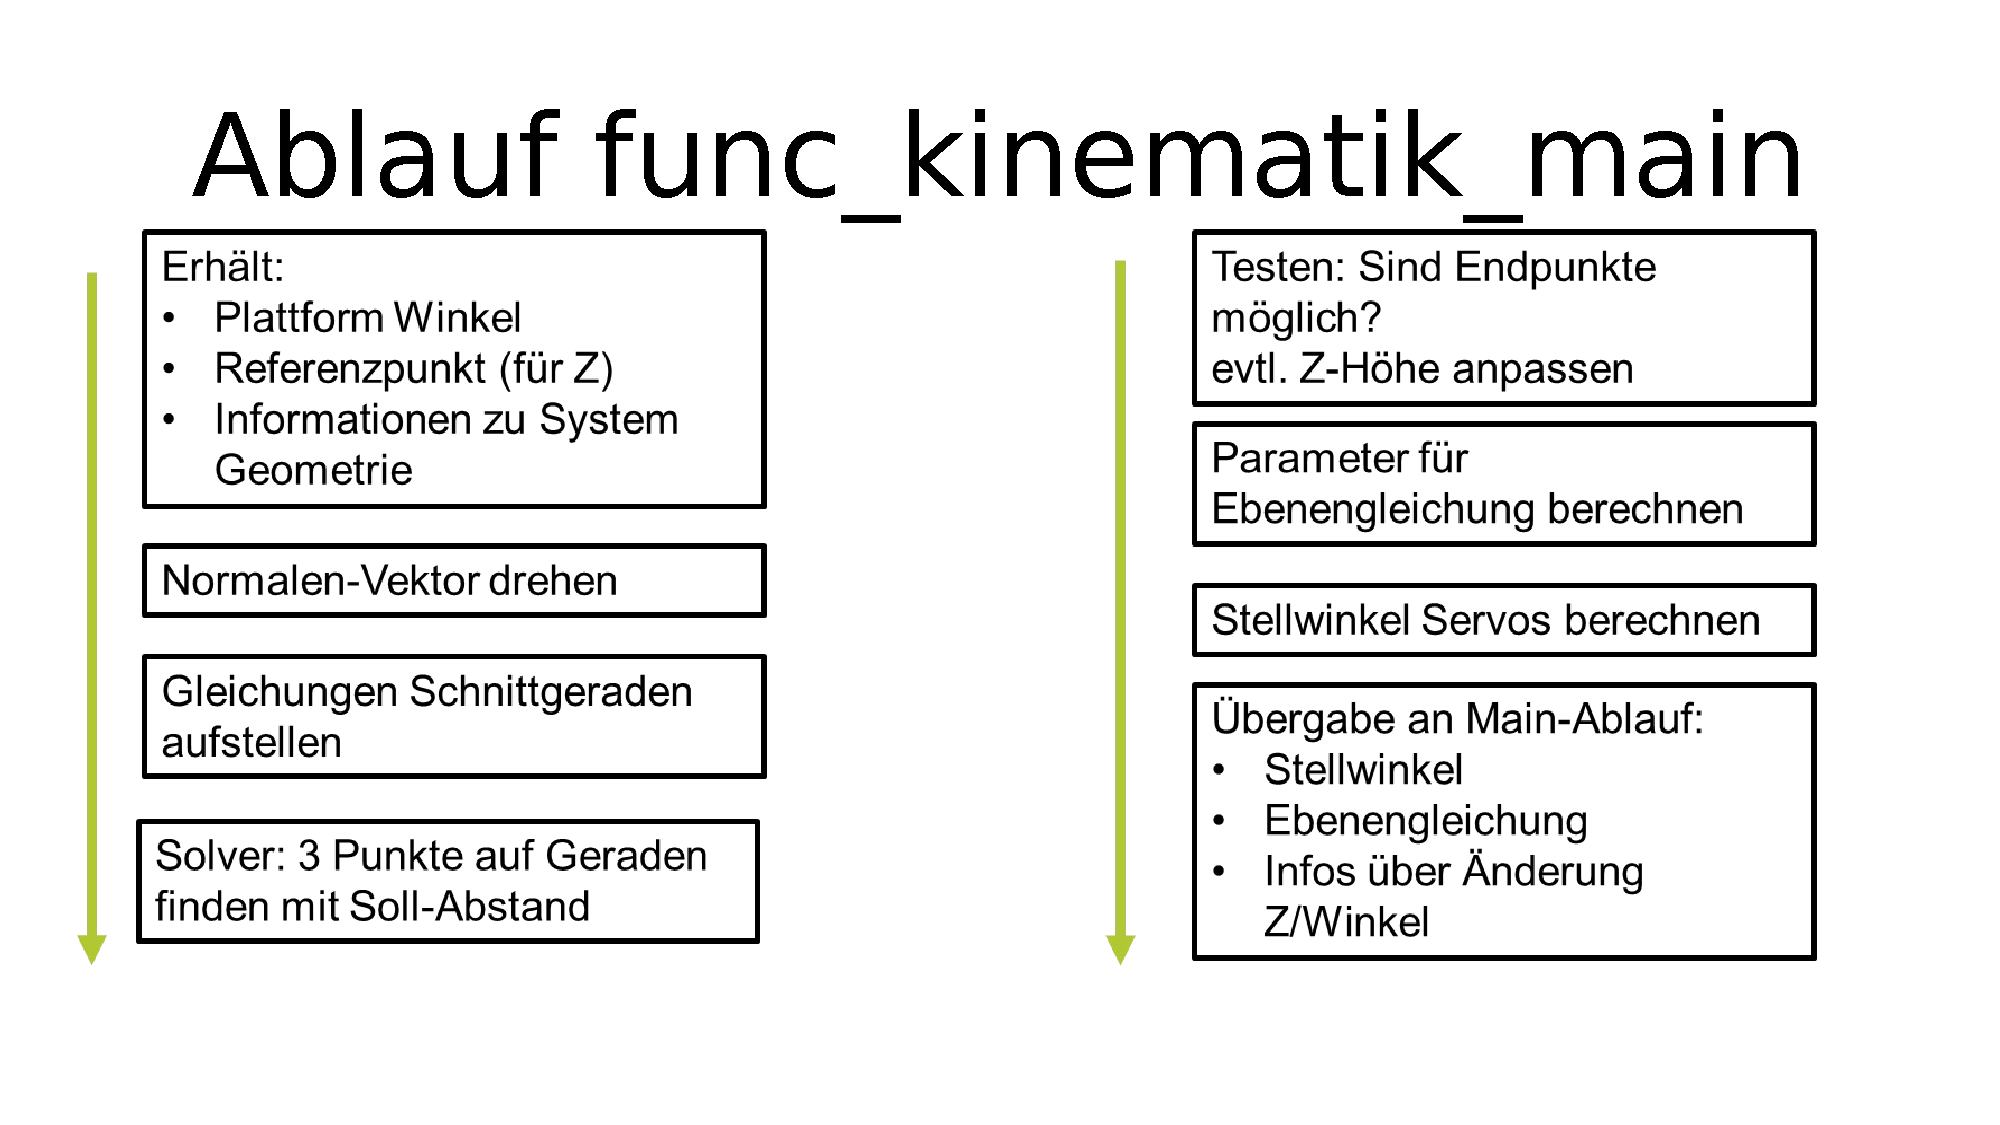
\includegraphics[width=0.7\textwidth]{Ablauf_kinematik.pdf}
  \caption{Prinzipieller Ablauf der Funktion zur Berechnung der Rückwärtskinematik}
  \label{fig:ablauf_kinematik}
\end{figure}

\section{Erreichbarkeit der Plattform}

Mit dem im vorherigen Kapitel beschriebenen Weg lässt sich die Plattform theoretisch in jede
Drehung und jede Höhe platzieren. Jedoch haben die Arme nur einen begrenzten
Bewegungsraum, was auch die möglichen Positionen der Plattform einschränkt. Sollte probiert
werden eine solche, nicht erreichbare Position anzufahren, kann nicht genau vorhergesehen
werden, in welcher Position die Plattform enden wird. Um dies zu vermeiden, wird in der Software
die Erreichbarkeit geprüft und gegebenenfalls angepasst. Die neuen Parameter werden dann
zurück übergeben.

Die erste Grenze des Bewegungsraums ist der Stellbereich des Servos. Dieser beträgt lediglich
180°, also kann auch der mit ihm verbundene untere Arm sich nur um 180° drehen.

Der nächste begrenzende Faktor ist die Gesamtlänge der Arme. Sind beide Arme ausgestreckt,
also in einer Linie, ist die maximale Entfernung erreicht. Sie entspricht der Länge beider Arme.
Wird dabei der Servo gedreht, ergibt sich so ein Kreis, der das äußere Limit der Arme beschreibt.

Eine maximale untere Grenze wird durch die Konstruktion des Roboters gegeben. Diese wird
deshalb als ein konstantes Limit über den Servowellen angenommen. Am Ende der Stellwege (0 und
180°) kann einfach der obere Arm gedreht werden, um beide Grenzen zu verbinden. Dies ergibt
dann den Bewegungsbereich, der in Abbildung~\ref{fig:bewegungsraum} zu sehen ist.

\begin{figure}[h]
  \centering
  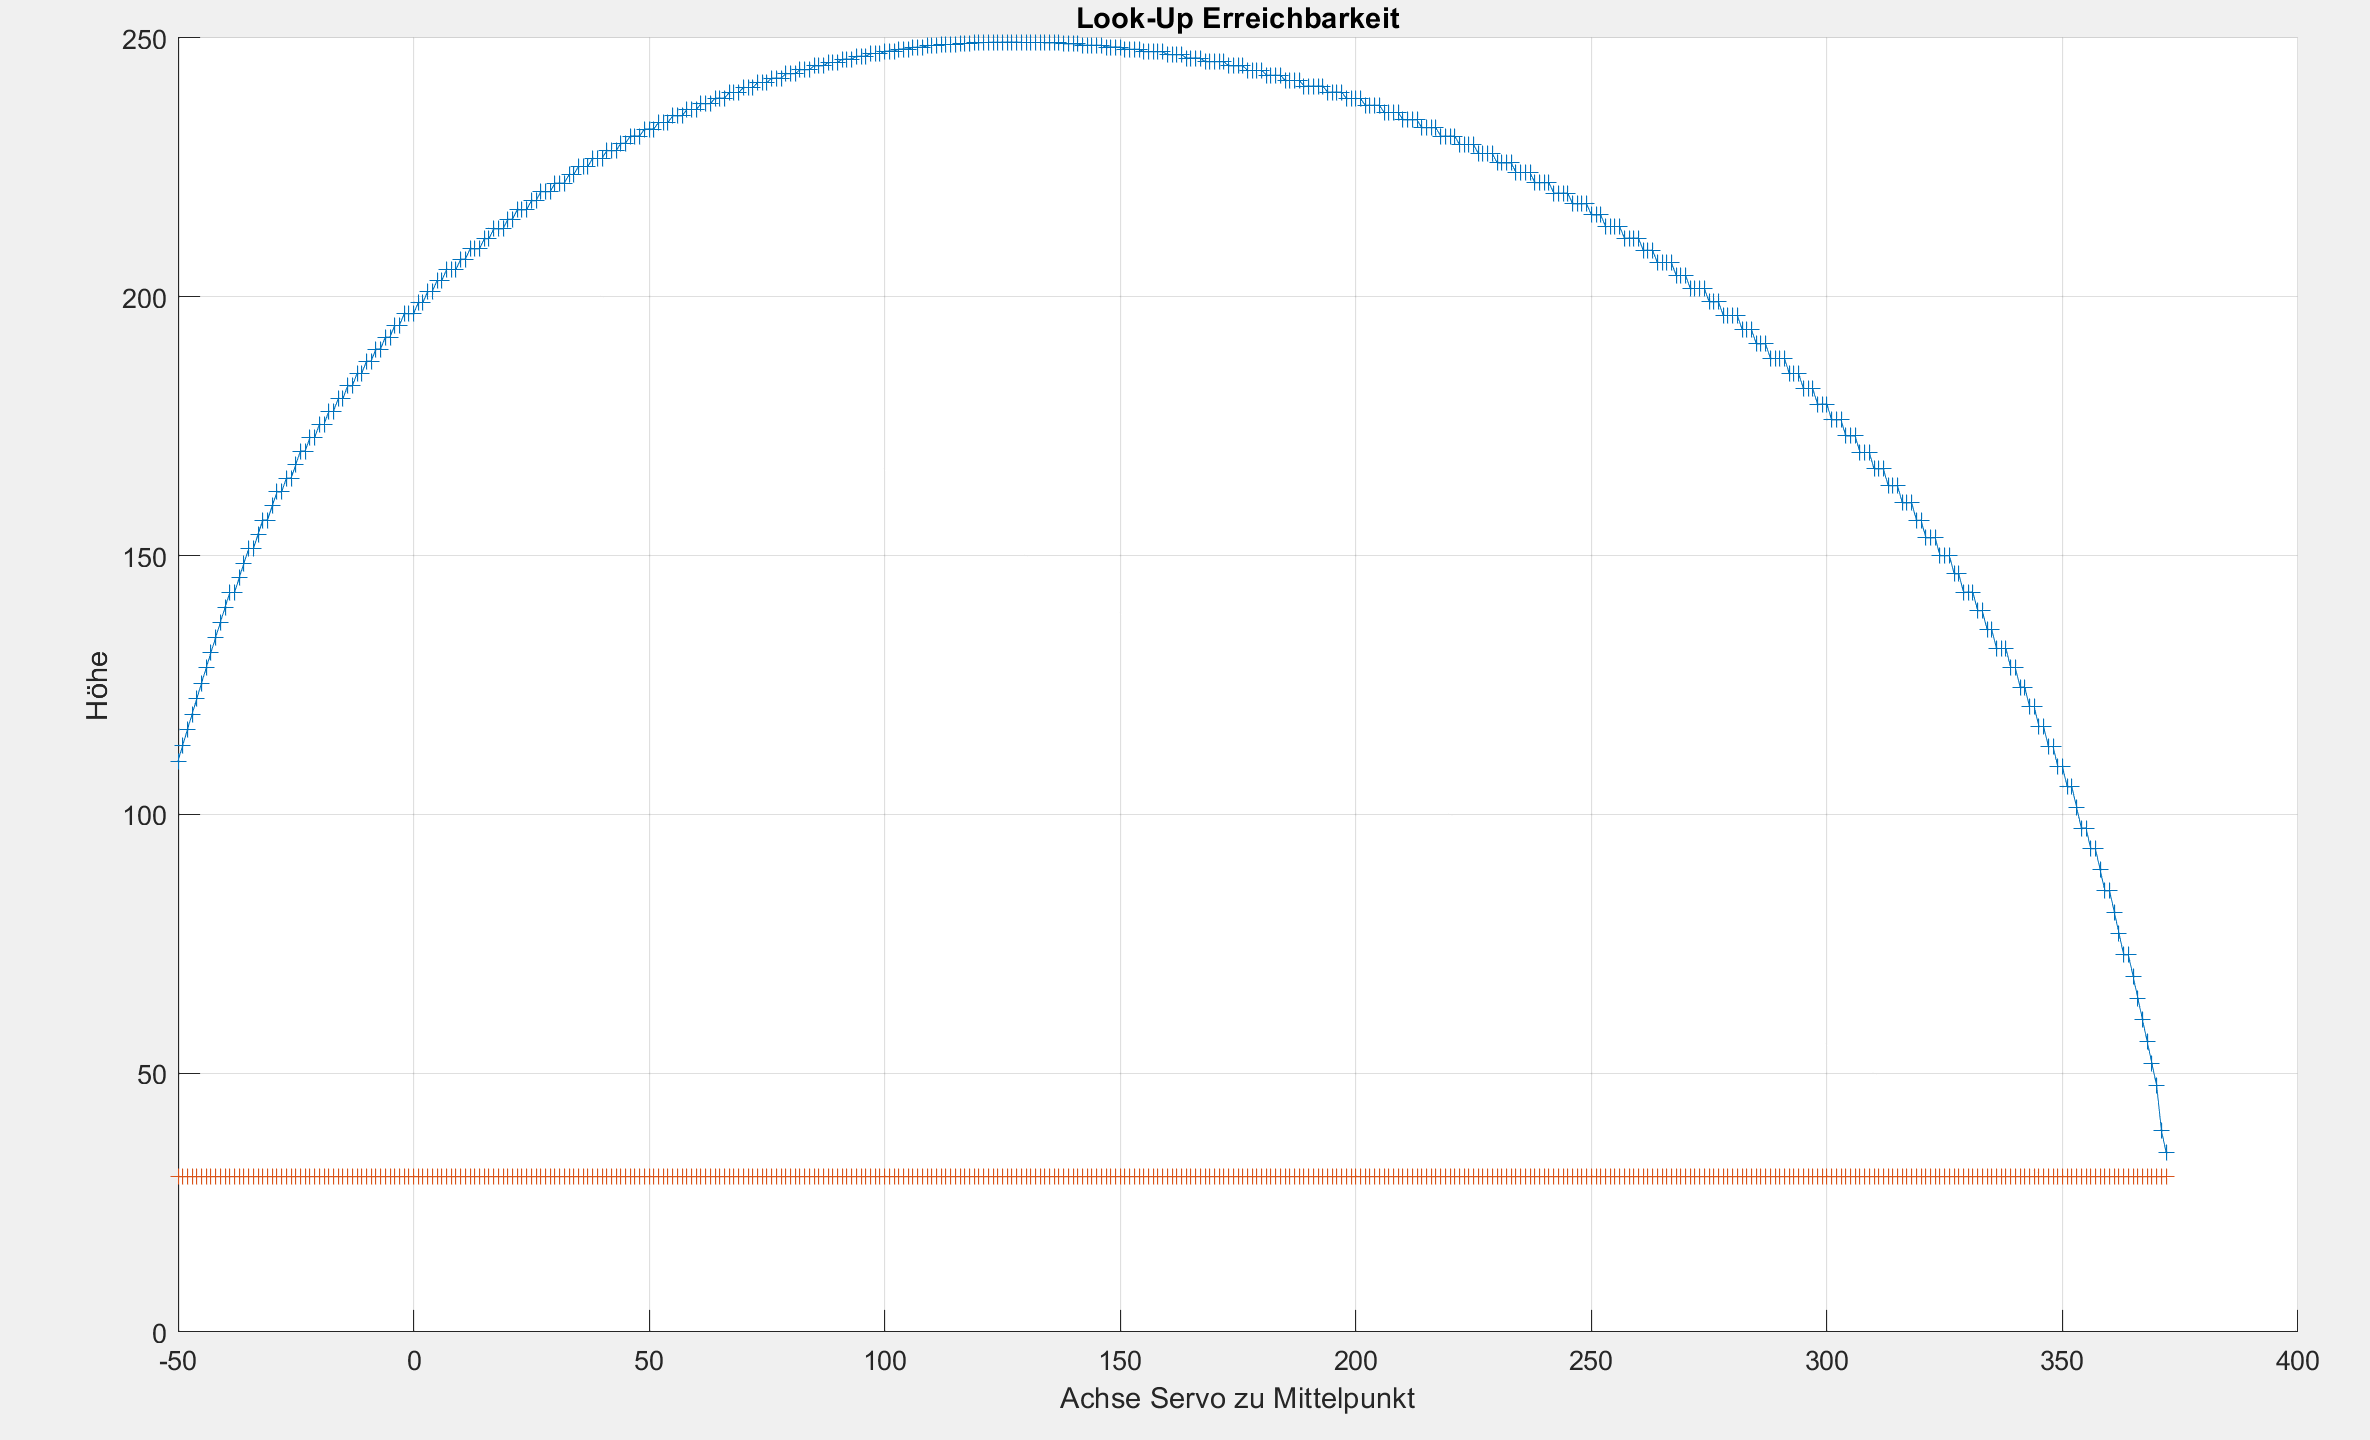
\includegraphics[width=0.85\textwidth]{Erreichbarkeit.png}
  \caption{Bewegungsraum der Arme}
  \label{fig:bewegungsraum}
\end{figure}

Zusätzlich muss noch beachtet werden, dass die beiden Arm-Elemente sich nur bis auf circa 20°
zueinander zusammenklappen können, sodass es auch einen Bereich um die Servowelle gibt, der
nicht erreichbar ist. Diese Bedingung lässt sich auch durch eine Mindestlänge zwischen Endpunkt
und Servowelle beschreiben. Da der Abstand in horizontaler Richtung durch die vorherigen
Berechnungen für die Plattform-Winkel festgelegt ist, ergibt sich eine Z-Höhe, bei der der
Endpunkt dann den Mindestabstand hätte.

Für die Software werden die Daten aus Abbildung~\ref{fig:bewegungsraum} als Look-Up-Table abgespeichert und
einmalig beim Start des Roboters in den Arbeitsspeicher geladen (\texttt{look\_up\_erreichbarkeit.mat}).
Nachdem potenzielle Endpunkte für eine Plattform berechnet wurden, können diese mit der
Funktion \texttt{func\_erreichbarkeit\_test} geprüft werden. Diese Funktion nutzt die zuvor beschriebene
Look-Up-Tabelle und die zusätzliche Mindestlänge, um zu prüfen, ob sich jeder Endpunkt im
erreichbaren Bereich befindet, indem sie deren Z-Höhe mit den Mini- und Maximalwerten für die
Koordinaten vergleicht. Sollte ein Arm außerhalb dieses Bereiches liegen, wird geprüft, ob durch
eine Verschiebung in Z-Richtung alle Arme erreichbar gemacht werden können. Ist dies der Fall,
schlägt die Funktion einen Z-Offset vor. Sollte dies nicht der Fall sein, weil z.\,B. der Winkel zu steil
ist, gibt die Funktion eine Warnung zurück.

\section{Errechnen der Servo-Stellwinkel}

Nachdem in den vorherigen Schritten die Plattform um die gewünschten Winkel gekippt und in
eine erreichbare Höhe platziert wurde, können nun für jeden Arm die Einstellwinkel der Servos
berechnet werden.

Dafür wird jeder Arm einzeln betrachtet und das System von einem räumlichen in ein ebenes
Problem überführt, wobei die neue waagerechte Achse dann die Gerade von Servowelle und
Ordinate ist. Die Senkrechte ist die Z-Richtung des originalen Systems.

\begin{figure}[h]
  \centering
  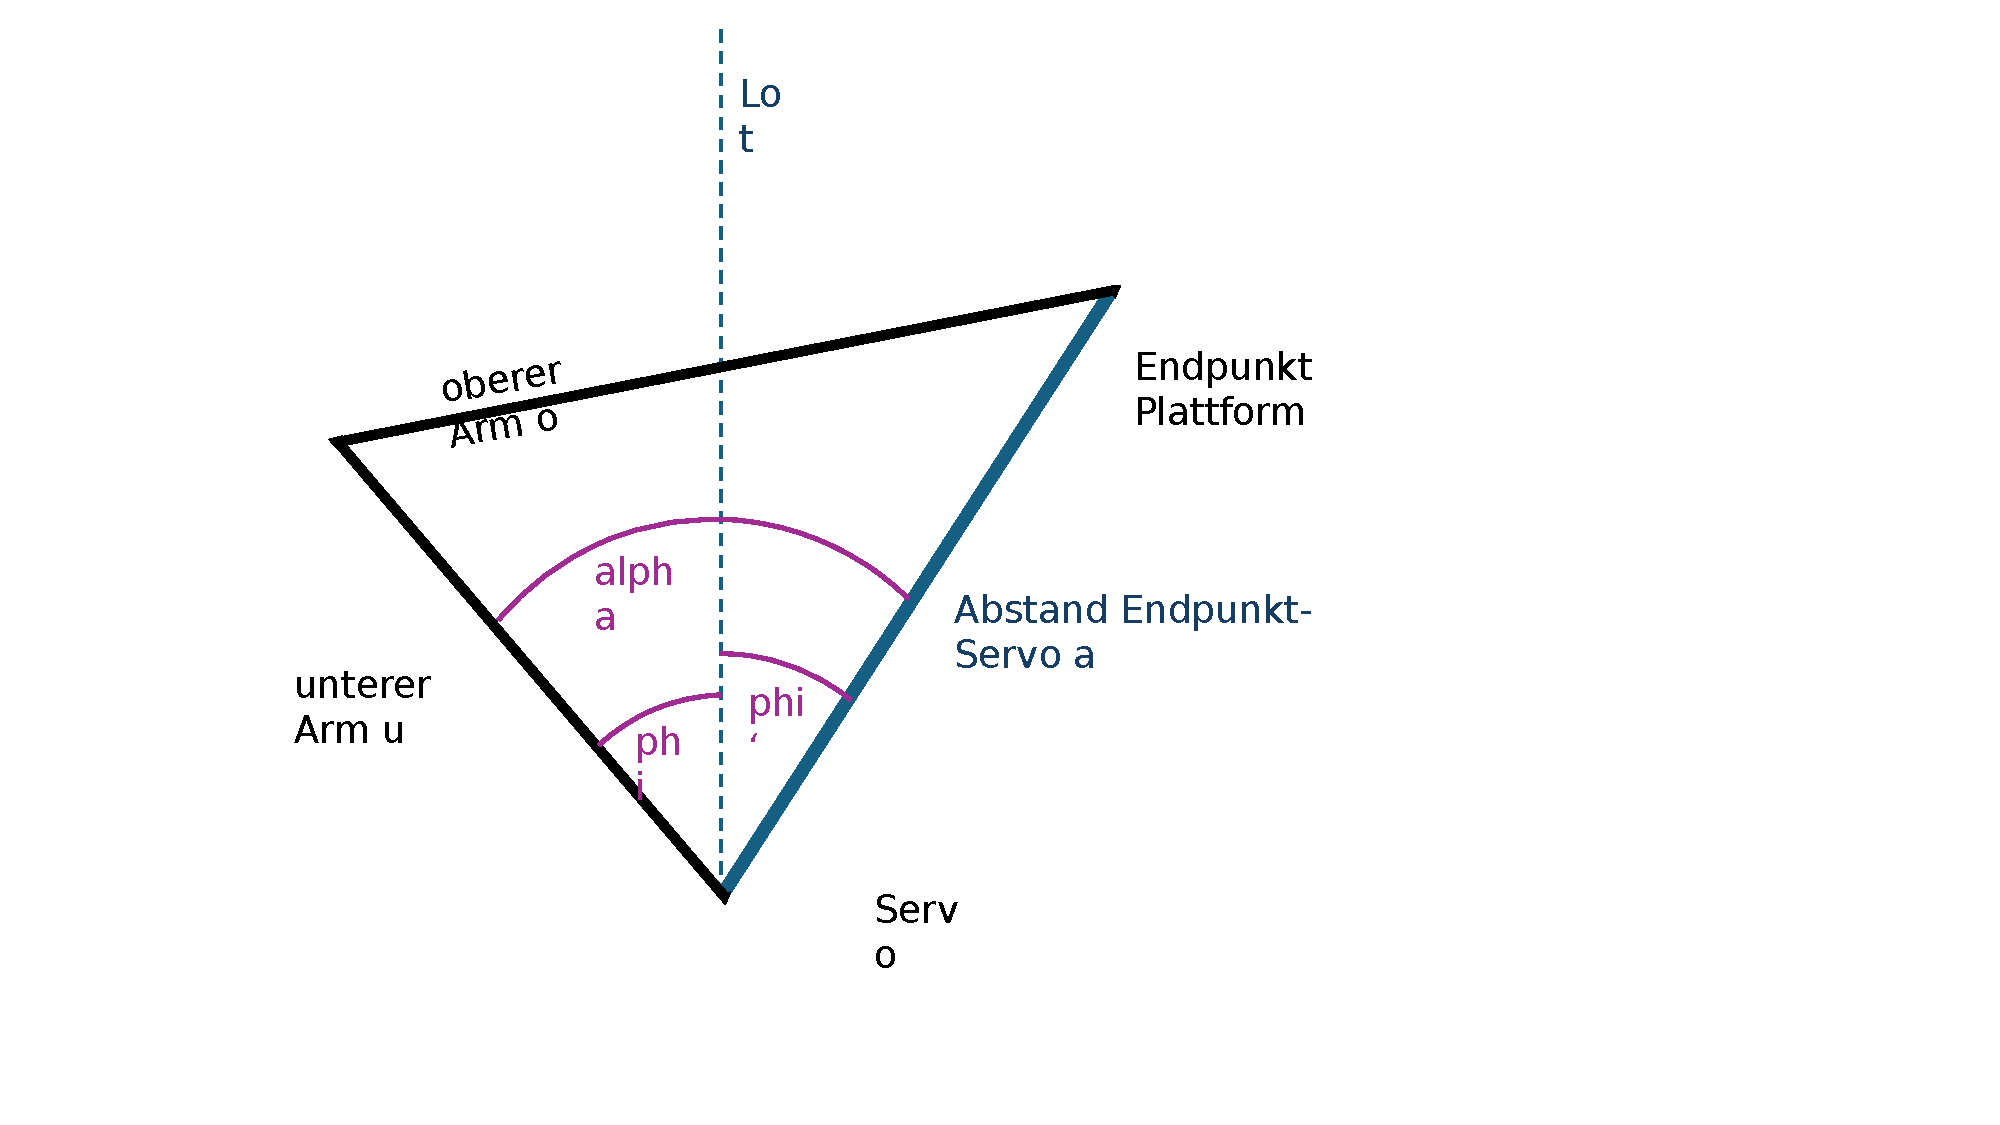
\includegraphics[width=0.6\textwidth]{Servo_Schaubild.pdf}
  \caption{Schaubild für die Rückwärtskinematik}
  \label{fig:schaubild_kinematik}
\end{figure}

Abbildung~\ref{fig:schaubild_kinematik} zeigt dieses 2D-System mit Blick auf die Servowelle. Die Lage des Plattform-Endpunktes sind aus den vorherigen Berechnungen bekannt. Die Position des Servos ist fix, somit
ist auch der Abstand Endpunkt-Servo bekannt, bzw. der Vektor, der diese Strecke beschreibt. Die
Längen der Arme sind auch konstant für diesen Roboter.

Somit lässt sich mit Hilfe des Kosinussatzes der Winkel $\alpha$ in diesem Dreieck berechnen.
Allerdings ist dieser Winkel noch nicht der Stellwinkel des Servos. Da die Nullposition des Servos
in der Lotgeraden angenommen wird, muss also noch der Winkel zwischen dem Lot und dem
Abstand Endpunkt-Servo abgezogen werden.

Mit der Funktion \texttt{func\_servo\_winkel} wird diese Berechnung für jeden Arm wiederholt. Diese gibt
dann einen Winkel in Grad, bezogen auf die Lotlinie, zurück.
Wie diese Winkel anschließend im Code an die Servos übertragen werden, ist in
Abschnitt~\ref{sec:hardware_abstraktion} beschrieben.

% ============================================================
\chapter{Computer Vision}


Damit der Roboter den Ball balancieren kann, muss er immer wissen, wo
der Ball gerade ist und in welche Richtung er sich bewegt. Diese Aufgabe
übernimmt die Computer-Vision-Komponente. Sie wertet das Kamerabild in
Echtzeit aus und liefert dem Regler die nötigen Informationen, damit dieser
die Plattform rechtzeitig in die richtige Richtung neigen kann.

Der Output besteht aus vier Werten: Position~$(x, y)$ und
Geschwindigkeit~$(v_x, v_y)$, jeweils in Pixeln bzw. Pixeln pro Sekunde,
relativ zur Bildmitte. Die Einordnung der CV-Komponente im Gesamtsystem
ist in Abbildung~\ref{fig:komponenten} dargestellt. In diesem Kapitel
wird erklärt, wie diese Werte berechnet werden und welche Überlegungen
hinter den einzelnen Designentscheidungen stecken.
Bearbeitet wurde dieser Teil von Leon Weyand.

\section{Kamerakalibrierung}

Die Kamera ist die einzige Informationsquelle des Systems über die Position
des Balls. Damit diese Informationen verlässlich sind, muss sie zuerst
kalibriert werden. Jede Kamera verzerrt das Bild ein bisschen, vor allem
an den Rändern, wo gerade Linien leicht gebogen wirken. Das hat einen
konkreten Effekt, denn ohne Kalibrierung weicht die gemessene Ballposition
leicht von der echten Position ab und der Regler würde dauerhaft mit
einem kleinen Fehler arbeiten.

Bei der Kalibrierung werden die sogenannten \textit{intrinsischen Parameter}
der Kamera bestimmt~\cite{intrinsic_parameters}. Dazu gehören die Kameramatrix, die beschreibt wie die
Kamera die dreidimensionale Welt auf das zweidimensionale Bild projiziert,
sowie die Verzerrungskoeffizienten, die die Linsenverzerrung mathematisch
beschreiben. Mit diesen Parametern lässt sich jedes aufgenommene Bild
anschließend rechnerisch entzerren.

\begin{figure}[h]
  \centering
  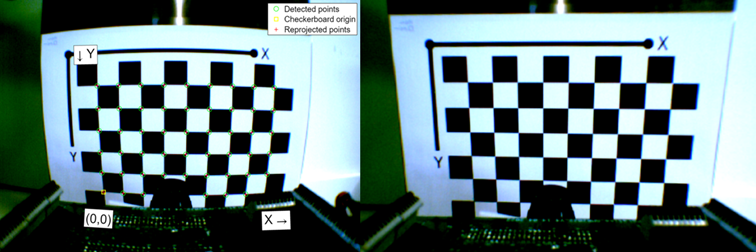
\includegraphics[width=0.85\textwidth]{Einfluss_der_Kamerakalibrierung.png}
  \caption{Kamerabild vor (links) und nach (rechts) der Entzerrung~\cite{hshl_kalibrierung}}
\end{figure}

Zur Kalibrierung wurde die klassische Schachbrettmethode verwendet,
die auch in der OpenCV-Bibliothek implementiert ist~\cite{opencv_calibration}. Die Idee dabei ist,
ein Schachbrettmuster aus mehreren verschiedenen Blickwinkeln zu
fotografieren. Da OpenCV die Ecken des Musters automatisch erkennt,
kann es daraus berechnen, wie die Kamera das Bild verzerrt.

Wichtig ist dabei, möglichst viele verschiedene Perspektiven abzudecken,
damit die Kalibrierung auch an den Bildrändern zuverlässig ist. Um das
ohne viel manuellen Aufwand zu erreichen, wurde der Aufnahmeprozess
direkt mit der Plattform automatisiert. Die Plattform kippt nacheinander
in sieben verschiedene Positionen (Mitte, links, rechts, vorne, hinten
und zwei Diagonalen), und die Kamera macht bei jeder Position automatisch
ein Foto. Das Schachbrett muss dabei nur einmal auf die Plattform gelegt werden,
den Rest erledigt das System von selbst. Die genauen Kippwinkel sind in
der Datei \texttt{positions.json} hinterlegt.

% Grafik: Foto des Schachbretts auf der Plattform
\begin{figure}[h]
  \centering
  \fbox{\parbox{0.5\textwidth}{\centering\vspace{20mm}
    [Foto: Schachbrettmuster auf der Plattform]
  \vspace{20mm}}}
  \caption{Schachbrettmuster auf der Plattform während der Kalibrierung}
\end{figure}

Das Ergebnis der Kalibrierung wird als \texttt{intrinsics.npz} gespeichert
und enthält die Kameramatrix sowie die Verzerrungskoeffizienten.
Als Qualitätsmaß gibt OpenCV den sogenannten RMS-Reprojektionsfehler aus,
der angibt wie genau die berechneten Parameter zum tatsächlichen Bild passen.
Je kleiner der Wert, desto besser. Die durchgeführte Kalibrierung erzielte
einen Fehler von unter 1 Pixel, was für die vorliegende Anwendung
ausreichend genau ist.


\section{Ballerkennung}

Der Ball muss in Echtzeit im Kamerabild gefunden werden.
Es wurde eine farbbasierte Methode gewählt, weil sie
schnell genug ist und zuverlässig funktioniert. Die Idee dahinter ist, im Bild alle Pixel zu suchen, die die Farbe
des Balls haben, und daraus den Mittelpunkt zu berechnen.

\subsection{Warum HSV statt RGB?}

Farben werden in Kameras normalerweise als RGB-Werte gespeichert, also als
Kombination aus Rot, Grün und Blau. Das Problem dabei ist, dass sich diese
Werte stark verändern, sobald sich die Beleuchtung ändert. Ein blauer
Ball sieht bei Tageslicht und bei Kunstlicht in RGB sehr unterschiedlich aus,
was einen stabilen Farbfilter schwer umsetzbar macht.

Der HSV-Farbraum (Hue, Saturation, Value, also Farbton, Sättigung und
Helligkeit) trennt diese Eigenschaften voneinander~\cite{opencv_colorspaces}. Der Farbton bleibt
dabei weitgehend unabhängig von der Beleuchtung. Da nach einem
blauen Ball gesucht wird, reicht es im HSV-Raum einen Bereich im Farbton
zu definieren, und der Filter funktioniert auch bei wechselnden
Lichtverhältnissen zuverlässig. Da ein blauer Ball verwendet wird,
wurden die HSV-Grenzwerte anhand typischer Standardwerte für Blau
gewählt und für die Lichtverhältnisse leicht angepasst.

\subsection{Erkennungs-Pipeline}

Die eigentliche Erkennung läuft in mehreren Schritten ab:


\begin{enumerate}
  \item \textbf{Farbraum-Umrechnung:} Das Kamerabild wird von BGR nach HSV umgerechnet.
  \item \textbf{Farbmaske:} Alle Pixel, deren HSV-Wert im definierten Farbbereich
        des Balls liegt, werden als weiß markiert; der Rest wird schwarz.
  \item \textbf{Rauschunterdrückung:} Ein Median-Filter glättet kleine Ausreißer,
        anschließend werden kleine isolierte Flecken durch morphologisches
        Opening und Closing entfernt~\cite{opencv_morphology}.
  \item \textbf{Größte Fläche:} Aus allen verbleibenden weißen Bereichen wird der
        größte ausgewählt. Das ist der Ball.
  \item \textbf{Kreisanpassung:} Um den gefundenen Bereich wird der kleinstmögliche
        Kreis gelegt. Sein Mittelpunkt ist die erkannte Ballposition.
\end{enumerate}

Damit ein Treffer als gültig gewertet wird, muss die gefundene Fläche
mindestens 500~Pixel² groß und der Radius mindestens 10~Pixel sein.
Diese Mindestgrenzen verhindern, dass Reflexionen oder Bildrauschen
fälschlicherweise als Ball erkannt werden.

\subsection{ROI-Tracking}

Statt in jedem Bild das gesamte Kamerabild nach dem Ball zu durchsuchen,
wird ROI-Tracking (Region of Interest) genutzt. Da der Ball sich zwischen
zwei Frames nur minimal bewegt, muss er im nächsten Bild ungefähr am gleichen
Ort sein wie im vorherigen. Gesucht wird deshalb nur noch in einem kleinen
Ausschnitt rund um die letzte bekannte Position.

Das reduziert den Rechenaufwand deutlich und erhöht die Erkennungsgeschwindigkeit.
Wird der Ball in diesem Ausschnitt fünfmal hintereinander nicht gefunden
(zum Beispiel weil er sich zu schnell bewegt hat), wird automatisch wieder
das gesamte Bild durchsucht und ein neuer Suchbereich festgelegt.
Der Grenzwert von fünf Fehlversuchen ist über den Parameter
\texttt{roi\_miss\_limit} konfigurierbar.

\subsection{Downsampling}

Zusätzlich zum ROI-Tracking wird das Suchfenster vor der Verarbeitung
auf eine kleinere Auflösung skaliert. Dadurch verringert sich die Anzahl der
zu verarbeitenden Pixel weiter, was die Detektionszeit deutlich reduziert.
Der dabei entstehende Genauigkeitsverlust ist für den Regelkreis vernachlässigbar.

\section{Videostream und Frame-Auswahl}
\label{sec:videostream}

Die Kamera liefert einen kontinuierlichen Videostream. Eine naive Umsetzung
würde bei jeder Anfrage einfach das nächste verfügbare Bild aus dem Puffer
lesen. Je nachdem wie schnell der Regler läuft und wie
voll der Puffer ist, könnte er ein Bild bekommen, das bereits mehrere
Frames alt ist. Der Ball hat sich in der Zwischenzeit vielleicht schon weiterbewegt.

Dieses Problem wird anders gelöst. Ein dedizierter Stream-Thread liest den
Videostream der Kamera in einer Endlosschleife und überschreibt dabei
kontinuierlich eine gemeinsame Variable mit dem jeweils neuesten Frame.
Alte Frames werden dabei implizit verworfen. Wenn der Regler ein Bild anfragt,
liest er genau diese Variable und erhält damit immer den aktuellsten Stand,
unabhängig davon, wann er fragt.

\begin{figure}[h]
  \centering
  \begin{tikzpicture}[
      node distance=2.2cm,
      box/.style={draw, rounded corners, minimum width=3cm, minimum height=1.2cm, align=center, fill=white},
      mem/.style={draw, rounded corners, minimum width=3cm, minimum height=1.2cm, align=center, fill=gray!10},
      arr/.style={-{Stealth}, thick},
    ]
    \node[box] (cam) {\textbf{Stream-Thread}\\{\small liest Videostream,}\\{\small verwirft alte Frames}};
    \node[mem, right=of cam] (buf) {\textbf{Aktuellstes Frame}\\{\small (gemeinsamer Speicher,}\\{\small Lock-gesichert)}};
    \node[box, right=of buf] (ctrl) {\textbf{Regel-Thread}\\{\small liest bei Bedarf}};

    \draw[arr] (cam) -- node[above]{\small schreibt} (buf);
    \draw[arr] (buf) -- node[above]{\small liest} (ctrl);

    \draw[arr, dashed] (cam.north) to[out=120,in=60,looseness=2]
      node[above]{\small kontinuierlich} (cam.north west);
  \end{tikzpicture}
  \caption{Stream-Thread und Regel-Thread greifen über einen gemeinsamen,
  Lock-gesicherten Speicherplatz auf das jeweils aktuellste Frame zu}
\end{figure}

Damit Stream-Thread und Regel-Thread nicht gleichzeitig auf denselben
Speicherplatz zugreifen, wird der Zugriff über ein Lock abgesichert. Ein Lock
stellt sicher, dass immer nur ein Thread gleichzeitig lesen oder schreiben darf.
So kann es nicht passieren, dass der Regler ein halb-überschriebenes Bild liest,
während der Stream-Thread gerade schreibt.


\section{Zustandsschätzung}

Die Klasse \texttt{BallTracker} bildet die Schnittstelle zwischen der
Bilderkennung und dem Regler. Sie kapselt intern einen
\texttt{BallDetectorRuntime} und erweitert dessen Ausgabe um eine
Geschwindigkeitsschätzung. Der Regler ruft ausschließlich
\texttt{BallTracker} auf und erhält als Antwort ein \texttt{BallState}-Objekt.

Alle Positionswerte beziehen sich auf ein einheitliches Koordinatensystem
mit dem Ursprung in der Bildmitte. Positive $x$-Richtung zeigt nach rechts,
positive $y$-Richtung nach oben. Die Werte werden in Pixeln angegeben.

Die Geschwindigkeit wird aus zwei aufeinanderfolgenden Messungen berechnet,
indem die Positionsänderung durch die vergangene Zeit geteilt wird:

\[
  v_x = \frac{x_{\text{neu}} - x_{\text{alt}}}{\Delta t}, \qquad
  v_y = \frac{y_{\text{neu}} - y_{\text{alt}}}{\Delta t}
\]

Zusätzlich wird der Betrag der Gesamtgeschwindigkeit berechnet:
$v = \sqrt{v_x^2 + v_y^2}$.

Wird kein Ball erkannt oder liegt noch keine vorherige Messung vor,
gibt \texttt{BallTracker} einen Zustand mit \texttt{valid = False} zurück.
Der Regler wertet dieses Flag aus und fährt die Plattform in diesem Fall
in die Neutralposition.

Der vollständige Ausgabe-Datensatz setzt sich wie folgt zusammen.

\begin{center}
\begin{tabular}{lll}
  \toprule
  Feld & Einheit & Bedeutung \\
  \midrule
  \texttt{x}, \texttt{y}     & px       & Position relativ zur Bildmitte \\
  \texttt{vx}, \texttt{vy}   & px/s     & Geschwindigkeit in X- und Y-Richtung \\
  \texttt{v}                 & px/s     & Betrag der Gesamtgeschwindigkeit \\
  \texttt{dt}                & s        & Zeit seit der letzten Messung \\
  \texttt{valid}             & Bool.    & \texttt{True} wenn Ball erkannt wurde \\
  \bottomrule
\end{tabular}
\end{center}


\section{Latenzmessung}

Damit der Regler stabil funktioniert, muss die Verarbeitungszeit der
CV-Komponente klein genug sein. Wenn die Erkennung zu langsam ist,
bekommt der Regler veraltete Informationen, weil der Ball sich schon
weiterbewegt hat, während der Regler noch auf die letzte Messung reagiert.
Die Latenz wurde deshalb auf dem Raspberry Pi in mehreren Entwicklungsstufen
gemessen und schrittweise optimiert. Dabei wird zwischen drei Phasen
unterschieden, die den Zeitraum der Detektion (\texttt{detect}),
den Bildabruf (\texttt{capture}) und die Farbraumkonvertierung
(\texttt{convert}) erfassen.

\textbf{Stufe 1 – Basisimplementierung ohne Optimierungen.}
In der ersten Messung wurde die Erkennung ohne ROI-Tracking und ohne
Downsampling betrieben. Jedes Bild wurde dabei per Einzelaufnahme von
der Kamera geholt. Tabelle~\ref{tab:latenz1} zeigt die gemessenen Werte.
Die Erkennung selbst dauerte im Mittel \SI{431,77}{\milli\second}, was
einer Bildrate von lediglich 2,22\,FPS entspricht. Damit war das System
für den Einsatz im Regelkreis noch nicht geeignet.

\begin{table}[h]
\centering
\caption{Latenzmessung Stufe 1 – ohne Optimierungen}
\label{tab:latenz1}
\begin{tabular}{lrrrr}
  \toprule
  Metrik & Mittelwert (ms) & Median (ms) & Min (ms) & Max (ms) \\
  \midrule
  capture & 18{,}22 & 17{,}38 & 14{,}14 & 40{,}95 \\
  convert & 0{,}16  & 0{,}01  & 0{,}01  & 5{,}72  \\
  detect  & 431{,}77 & 425{,}71 & 389{,}79 & 510{,}75 \\
  total   & 450{,}15 & 444{,}58 & 404{,}13 & 527{,}43 \\
  \midrule
  \multicolumn{2}{l}{Geschätzte FPS (Mittelwert)} & \multicolumn{3}{r}{2{,}22} \\
  \bottomrule
\end{tabular}
\end{table}

\textbf{Stufe 2 – ROI-Tracking und Downsampling.}
Durch die Einführung von ROI-Tracking und Downsampling konnte die
Detektionszeit drastisch reduziert werden. Die Kamera wurde weiterhin
per Einzelaufnahme abgefragt. Die Ergebnisse sind in
Tabelle~\ref{tab:latenz2} dargestellt. Die Detektionszeit sank auf
im Mittel \SI{62,87}{\milli\second}, die Gesamtlatenz auf
\SI{82,63}{\milli\second}, was einer Bildrate von 12,10\,FPS entspricht.

\begin{table}[h]
\centering
\caption{Latenzmessung Stufe 2 – mit ROI-Tracking und Downsampling}
\label{tab:latenz2}
\begin{tabular}{lrrrr}
  \toprule
  Metrik & Mittelwert (ms) & Median (ms) & Min (ms) & Max (ms) \\
  \midrule
  capture & 19{,}76 & 17{,}87 & 14{,}20 & 43{,}29 \\
  convert & 0{,}01  & 0{,}01  & 0{,}01  & 0{,}02  \\
  detect  & 62{,}87 & 62{,}36 & 60{,}56 & 90{,}73 \\
  total   & 82{,}63 & 80{,}81 & 75{,}09 & 112{,}26 \\
  \midrule
  \multicolumn{2}{l}{Geschätzte FPS (Mittelwert)} & \multicolumn{3}{r}{12{,}10} \\
  \bottomrule
\end{tabular}
\end{table}

\textbf{Stufe 3 – Stream-Thread statt Einzelaufnahmen.}
In der finalen Implementierung wird die Kamera nicht mehr per Einzelaufnahme
abgefragt, sondern über den in Abschnitt~\ref{sec:videostream} beschriebenen
Stream-Thread betrieben. Da dieser den Videostream kontinuierlich liest und
immer nur das aktuellste Frame vorhält, entfällt der Overhead der
Kamerainitialisierung bei jedem Bildabruf.
% ============================================================
\chapter{Regelung}

In diesem Kapitel wird die Auslegung und Implementierung der Positionsregelung für den Ball-Balancing-Roboter beschrieben. Ursprünglich war ein reiner PD-Regler vorgesehen, jedoch zeigte sich in der physikalischen Modellierung und späteren Praxis schnell, dass ein I-Anteil zwingend erforderlich ist, um stationäre Regelabweichungen durch asymmetrische Reibung zu kompensieren. Die Entwicklung gliedert sich in die Aufbereitung der Sensordaten, die analytische Reglerauslegung, die Verifikation in der Simulation sowie die finale hardwarenahe Implementierung. Bearbeitet wurde dieser Teil von Hanan Jawesh.

\section{Koordinatentransformation des Kamerabildes}

Bevor die Kameradaten im Regelkreis verwendet werden können, muss sichergestellt werden, dass das zweidimensionale Koordinatensystem der Kamera exakt mit dem physikalischen Koordinatensystem der Aktuatorik übereinstimmt. Eine mechanische Fehlstellung der Kamera führt zu einer unerwünschten Kreuzkopplung der X- und Y-Achsen im Regler.

Um dies zu korrigieren, wurde eine softwareseitige Rotationskorrektur implementiert. Das System wird kalibriert, indem der Ball physikalisch ausschließlich entlang der positiven Y-Achse bewegt wird. Aus den vom Vision-System erfassten Pixelkoordinaten des Start- und Endpunktes ($p_1$ und $p_2$) lässt sich der Fehlwinkel der Kamera berechnen. Der aktuelle Winkel des Bewegungsvektors im Kamerabild berechnet sich zu:
\begin{equation}
    \theta_{\text{ist}} = \text{atan2}(p_{2,y} - p_{1,y}, p_{2,x} - p_{1,x})
\end{equation}
Da die physische Bewegung exakt auf der Y-Achse ($90^\circ$ bzw. $\frac{\pi}{2}$) stattfand, ergibt sich der benötigte Rotationswinkel zur Korrektur aus $\Delta\theta = \frac{\pi}{2} - \theta_{\text{ist}}$.
Jede neu erfasste Position $(x, y)$ sowie die ermittelten Geschwindigkeiten $(v_x, v_y)$ werden in Echtzeit über eine 2D-Rotationsmatrix um den Bildmittelpunkt gedreht:
\begin{equation}
    \begin{pmatrix} x_{\text{korr}} \\ y_{\text{korr}} \end{pmatrix} =
    \begin{pmatrix} \cos(\Delta\theta) & -\sin(\Delta\theta) \\ \sin(\Delta\theta) & \cos(\Delta\theta) \end{pmatrix}
    \begin{pmatrix} x \\ y \end{pmatrix}
\end{equation}
Diese Transformation entkoppelt die Achsen und garantiert, dass ein Stellsignal des Reglers in X-Richtung ausschließlich eine Bewegung der Plattform in X-Richtung nach sich zieht.

\section{Systemmodellierung und analytische Reglerauslegung}

Um die optimalen Parameter für den Regler analytisch bestimmen zu können, muss die Regelstrecke zunächst mathematisch modelliert werden. Eine Kugel, die auf einer geneigten Ebene rollt, erfährt nicht die volle Erdbeschleunigung, da ein Teil der potentiellen Energie in Rotationsenergie übergeht.

Für eine Vollkugel mit der Masse $m$, dem Radius $r$ und dem Trägheitsmoment $J = \frac{2}{5} m r^2$ ergibt sich aus dem Drallsatz und dem Newtonschen Aktionsprinzip die lineare Beschleunigung $a$ in Abhängigkeit des Neigungswinkels $\alpha$:
\begin{equation}
    a = g \cdot \sin(\alpha) \cdot \left( \frac{m}{m + \frac{J}{r^2}} \right) = \frac{5}{7} g \cdot \sin(\alpha)
\end{equation}
Für kleine Auslenkwinkel lässt sich die Übertragungsfunktion linearisieren ($\sin(\alpha) \approx \alpha$). Damit verhält sich die Strecke wie ein doppelter Integrator. Im Laplace-Raum lautet die Übertragungsfunktion der Strecke $P(s)$ somit:
\begin{equation}
    P(s) = \frac{X(s)}{\alpha(s)} = \frac{K_{\text{sys}}}{s^2} \quad \text{mit} \quad K_{\text{sys}} = \frac{5}{7}g
\end{equation}
Für die Auslegung eines PD-Reglers mit der Übertragungsfunktion $C(s) = K_p + K_d s$ ergibt sich die geschlossene Übertragungsfunktion des Regelkreises $T(s)$ zu:
\begin{equation}
    T(s) = \frac{P(s)C(s)}{1 + P(s)C(s)} = \frac{K_{\text{sys}} (K_d s + K_p)}{s^2 + K_{\text{sys}} K_d s + K_{\text{sys}} K_p}
\end{equation}
Nach der Methode der Polvorgabe~\cite{unbehauen2008} wird das Nennerpolynom mit der charakteristischen Gleichung eines idealen Verzögerungsgliedes zweiter Ordnung gleichgesetzt:
\begin{equation}
    s^2 + K_{\text{sys}} K_d s + K_{\text{sys}} K_p = s^2 + 2\zeta\omega_n s + \omega_n^2
\end{equation}
Durch Koeffizientenvergleich lassen sich die optimalen Reglerparameter $K_p$ und $K_d$ in Abhängigkeit der gewünschten Dynamik direkt berechnen:
\begin{equation}
    K_p = \frac{\omega_n^2}{K_{\text{sys}}}, \quad K_d = \frac{2\zeta\omega_n}{K_{\text{sys}}}
\end{equation}
Für ein ballbalancierendes System wird ein aperiodischer Grenzfall gewählt ($\zeta = 1{,}0$), um ein Überschwingen der Kugel über den Sollwert zu verhindern. Die Eigenkreisfrequenz $\omega_n$ ist durch die Abtastrate des Systems limitiert und wurde anwendungsspezifisch gewählt.

Da die reale Strecke durch Coulombsche Reibung und Haftreibung gestört wird, bleibt der Ball bei kleinen Positionsfehlern stehen. Der Regler wurde daher empirisch um einen Integralanteil ($K_i$) erweitert, der diese konstanten Störgrößen ausregelt.

\section{Simulation in MATLAB/Simulink}

Vor der Implementierung auf der Hardware wurde der Regler in MATLAB/Simulink verifiziert. Das Modell bildet die Nichtlinearitäten der Strecke (Haft- und Rollreibung) sowie Signaltotzeiten explizit ab.

\begin{figure}[h]
    \centering
    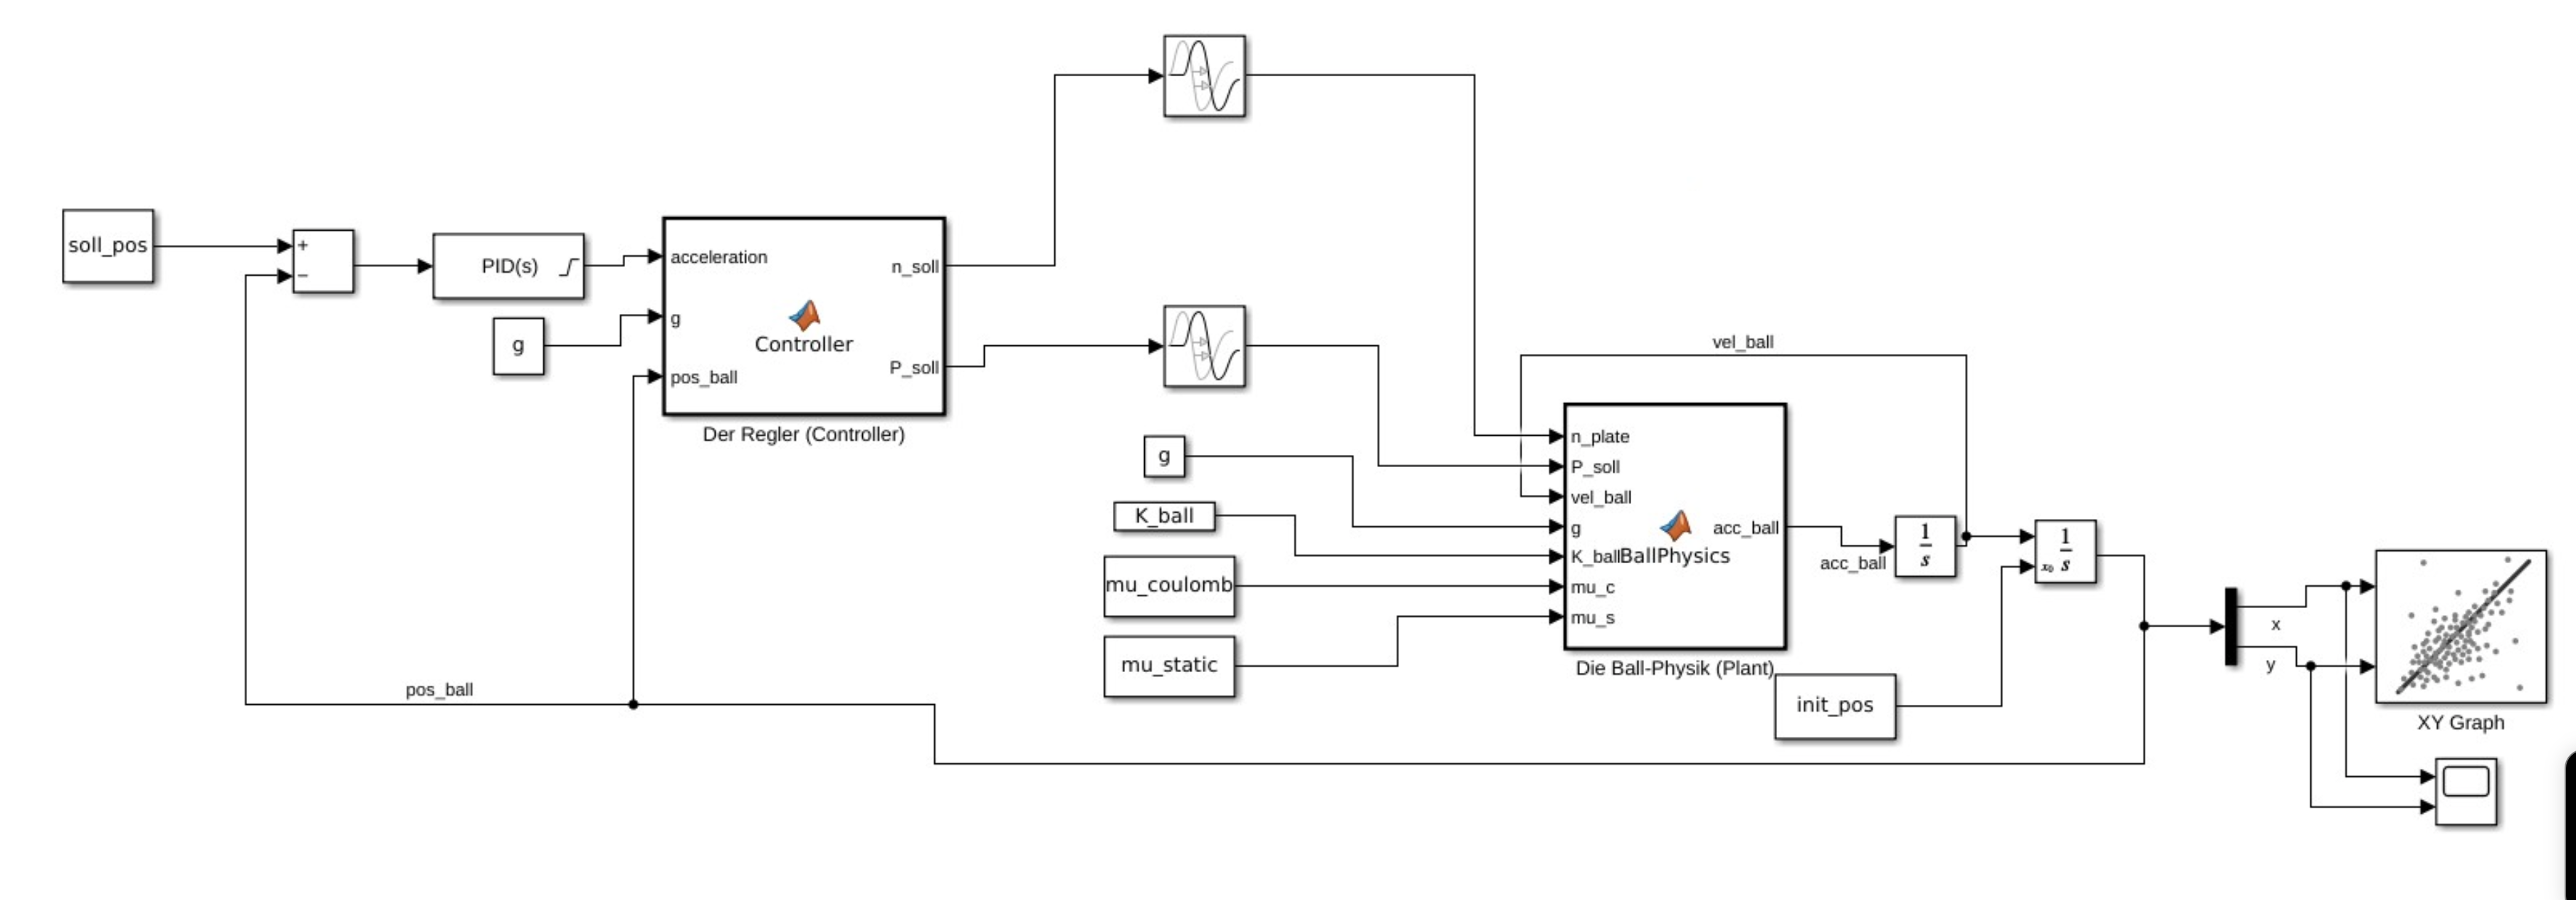
\includegraphics[width=0.9\textwidth]{simulink_blockdiagramm.png}
    \caption{Vollständiges Blockschaltbild der MATLAB/Simulink-Simulation inklusive Regler, Streckenmodell und Totzeitgliedern}
    \label{fig:simulink_modell}
\end{figure}

Die Simulation wurde mit einer festen Schrittweite von \SI{0{,}02}{\second} parametriert, was einer Arbeitsfrequenz von \SI{50}{\hertz} entspricht. Tests mit geringeren Frequenzen zeigten einen drastischen Stabilitätsverlust, was die geforderte Abtastrate physikalisch legitimiert.

Um den Windup-Effekt des Integrators zu verhindern, wurde eine Limitierung (Clamping) implementiert. Überschreitet das Reglersignal eine Ausgangsbeschleunigung von $\pm\SI{2{,}5}{\metre\per\second\squared}$, wird die Integration gestoppt. Zusätzlich wurde eine Systemtotzeit von \SI{4}{\milli\second} eingefügt, um die Signalverarbeitungsdauer zu den PWM-Treibern realitätsnah abzubilden.

\begin{figure}[h]
    \centering
    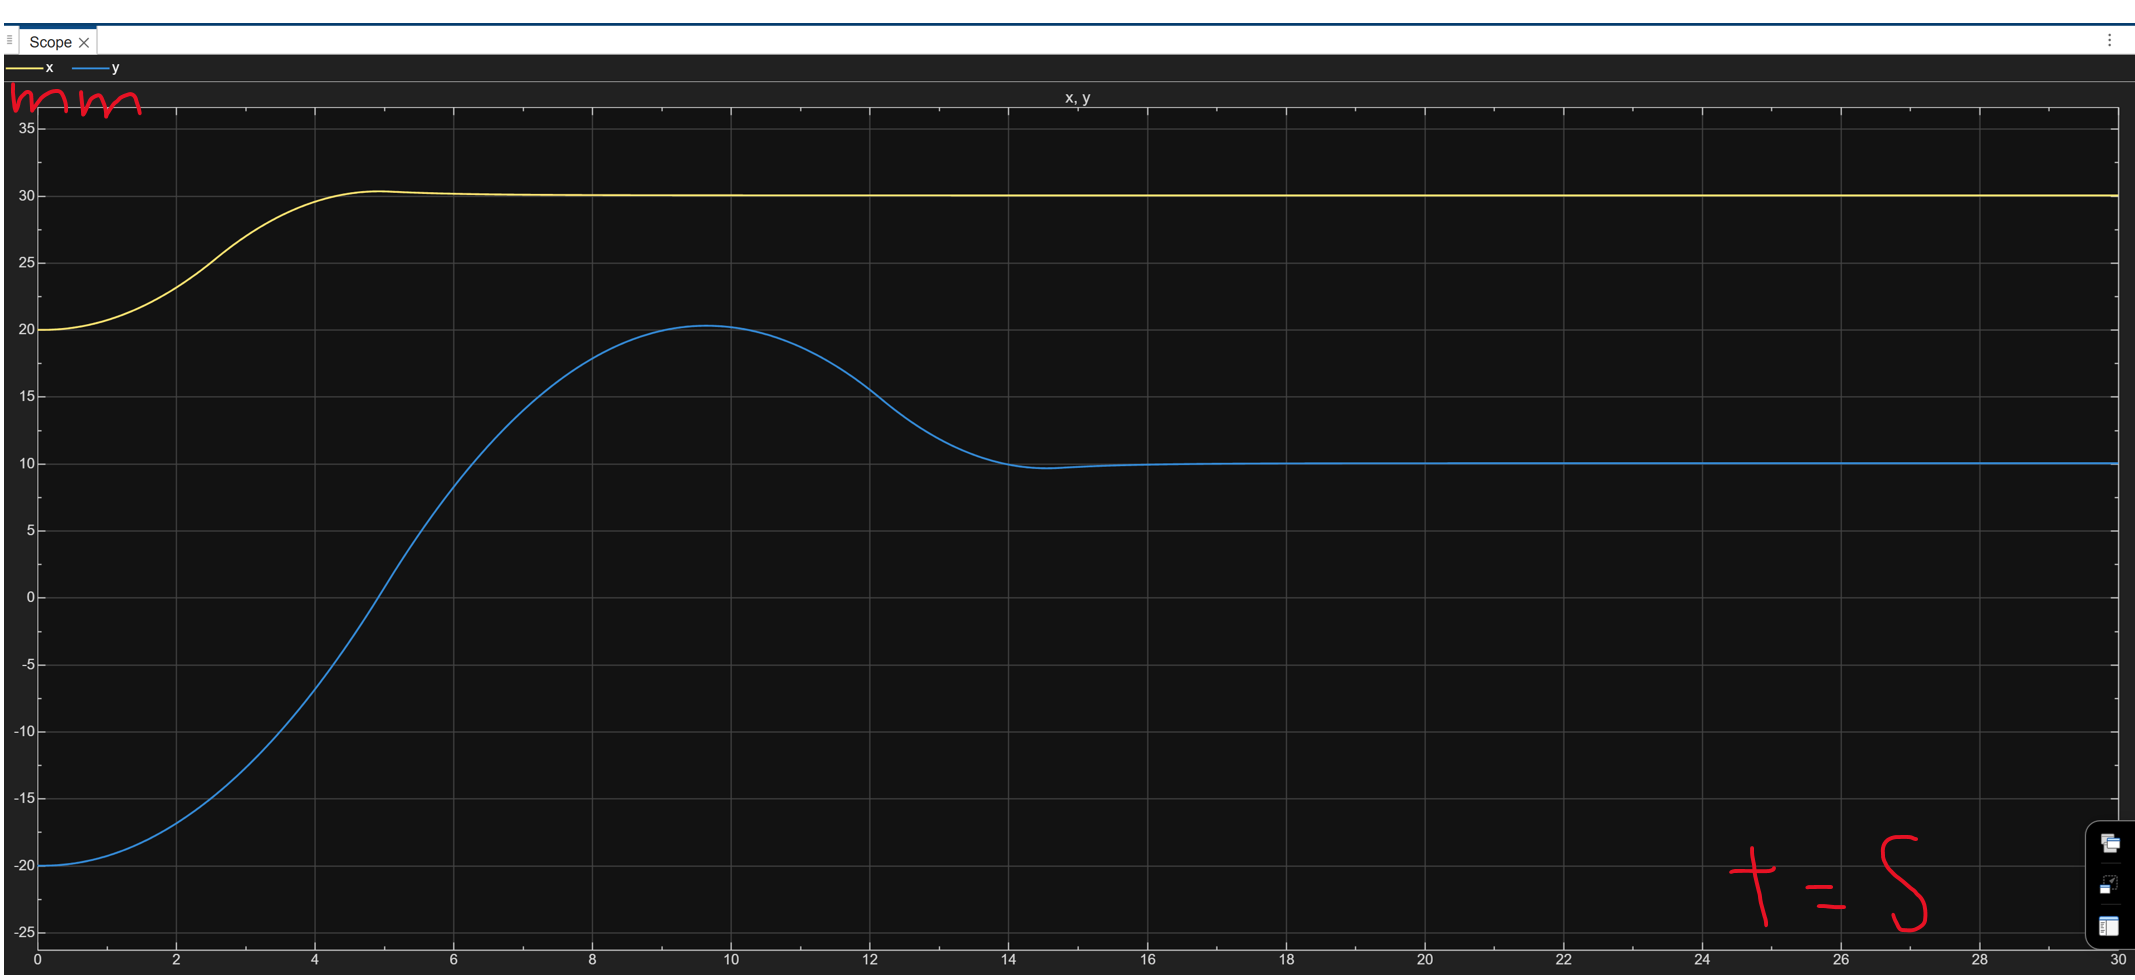
\includegraphics[width=0.8\textwidth]{sprungantwort_scope.png}
    \caption{Simulierte Sprungantwort des geregelten Systems auf der X- und Y-Achse bei \SI{50}{\hertz} Abtastrate}
    \label{fig:sprungantwort}
\end{figure}

Die simulierte Sprungantwort (Abbildung~\ref{fig:sprungantwort}) zeigt ein robustes Einregelverhalten der Kugel auf den gewünschten Sollwert ohne Dauerschwingung.

\section{Diskreter Regelloop und Hardware-Implementierung}

Die validierte Reglerstruktur wurde als zeitdiskreter Algorithmus in Python portiert. Der PID-Regler läuft in \texttt{main\_control.py} in einer definierten Zeitschleife. Er berechnet aus der Positionsabweichung und der aktuellen Geschwindigkeit die benötigten Beschleunigungswerte $a_{x,\text{req}}$ und $a_{y,\text{req}}$. Die Geschwindigkeit wird dabei als negativer D-Anteil genutzt, um den Derivative Kick bei Sollwertsprüngen zu vermeiden.

Diese Vorgaben werden auf maximal $\pm\SI{5{,}0}{\metre\per\second\squared}$ begrenzt, was ca. $30^\circ$ Plattenneigung entspricht, und anschließend an die Kinematik übergeben. Dort werden die Beschleunigungen in die benötigten Kippwinkel der Plattform umgerechnet:
\begin{equation}
    \theta_x = -\arcsin\!\left(\frac{a_{y,\text{req}}}{g}\right), \quad \theta_y = \arcsin\!\left(\frac{a_{x,\text{req}}}{g}\right)
\end{equation}
Diese Winkel dienen der inversen Kinematik als Eingabe, um die Stellwinkel der drei Servomotoren zu berechnen. Damit ist der vollständige Regelkreis von der visuellen Erfassung des Balls bis zur mechanischen Reaktion der Servomotoren geschlossen.

\begin{thebibliography}{9}

\bibitem{opencv_calibration}
OpenCV Documentation.
\textit{Camera Calibration}.
\url{https://docs.opencv.org/4.x/dc/dbb/tutorial_py_calibration.html}

\bibitem{hshl_kalibrierung}
HSHL Wiki.
\textit{Einfluss der Kamerakalibrierung}.
\url{https://wiki.hshl.de/wiki/index.php/Datei:Einfluss_der_Kamerakalibrierung.png}

\bibitem{opencv_colorspaces}
OpenCV Documentation.
\textit{Changing Colorspaces}.
\url{https://docs.opencv.org/4.x/df/d9d/tutorial_py_colorspaces.html}

\bibitem{opencv_morphology}
OpenCV Documentation.
\textit{Morphological Transformations}.
\url{https://docs.opencv.org/4.x/d9/d61/tutorial_py_morphological_ops.html}

\bibitem{unbehauen2008}
H. Unbehauen.
\textit{Regelungstechnik I: Klassische Verfahren zur Analyse und Synthese linearer kontinuierlicher Regelsysteme}, 15.~Auflage.
Vieweg+Teubner Verlag, 2008.

\bibitem{intrinsic_parameters}
ShadeCoder.
\textit{Intrinsic Parameters: A Comprehensive Guide for 2025}.
\url{https://www.shadecoder.com/de/topics/intrinsic-parameters-a-comprehensive-guide-for-2025}

\end{thebibliography}

% ============================================================
\appendix
\chapter{Zeichnungssatz Mechanische Baugruppe}
\label{app:zeichnungen}

Der folgende Zeichnungssatz wurde von Simon Bernarding erstellt und enthält die Fertigungszeichnungen aller mechanischen Bauteile des Balancing Robots.

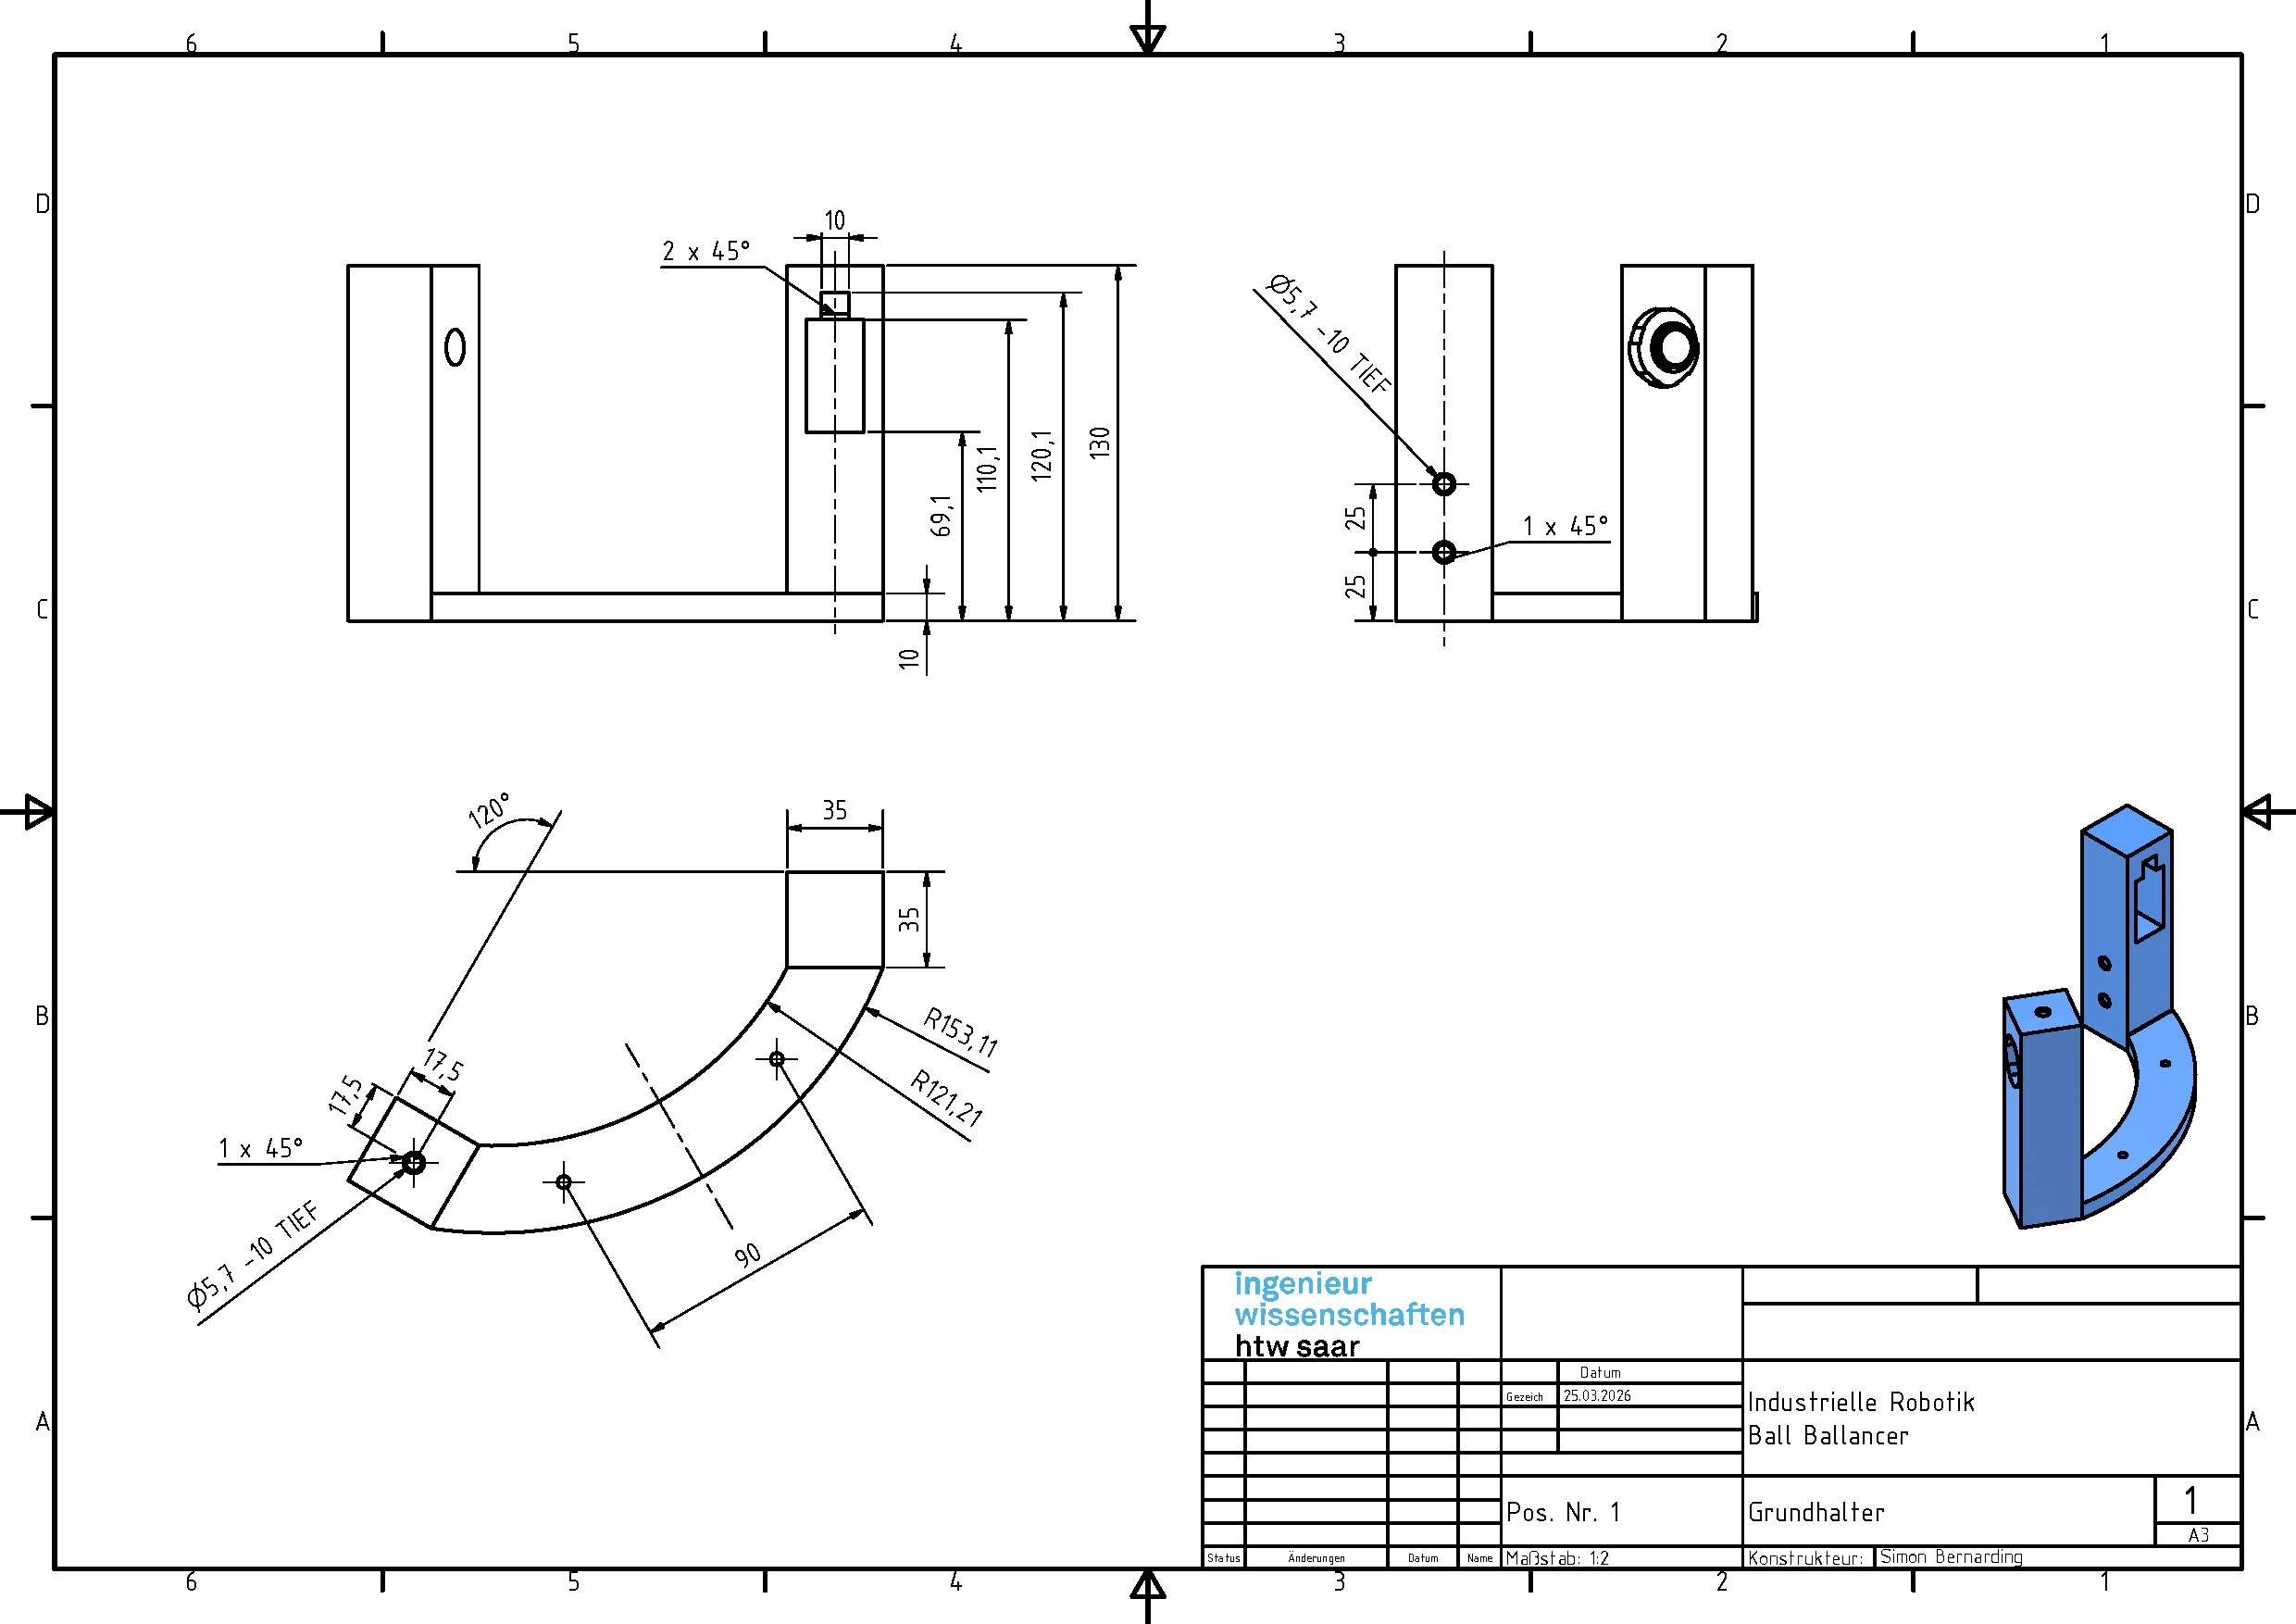
\includepdf[pages=-]{Zeichnungssatz_Bernarding.pdf}

\chapter{Baugruppenzeichnung Technikbox}
\label{app:technikbox}

Die folgende Zeichnung zeigt den Gesamtaufbau der Technikbox mit allen integrierten Elektronikkomponenten.

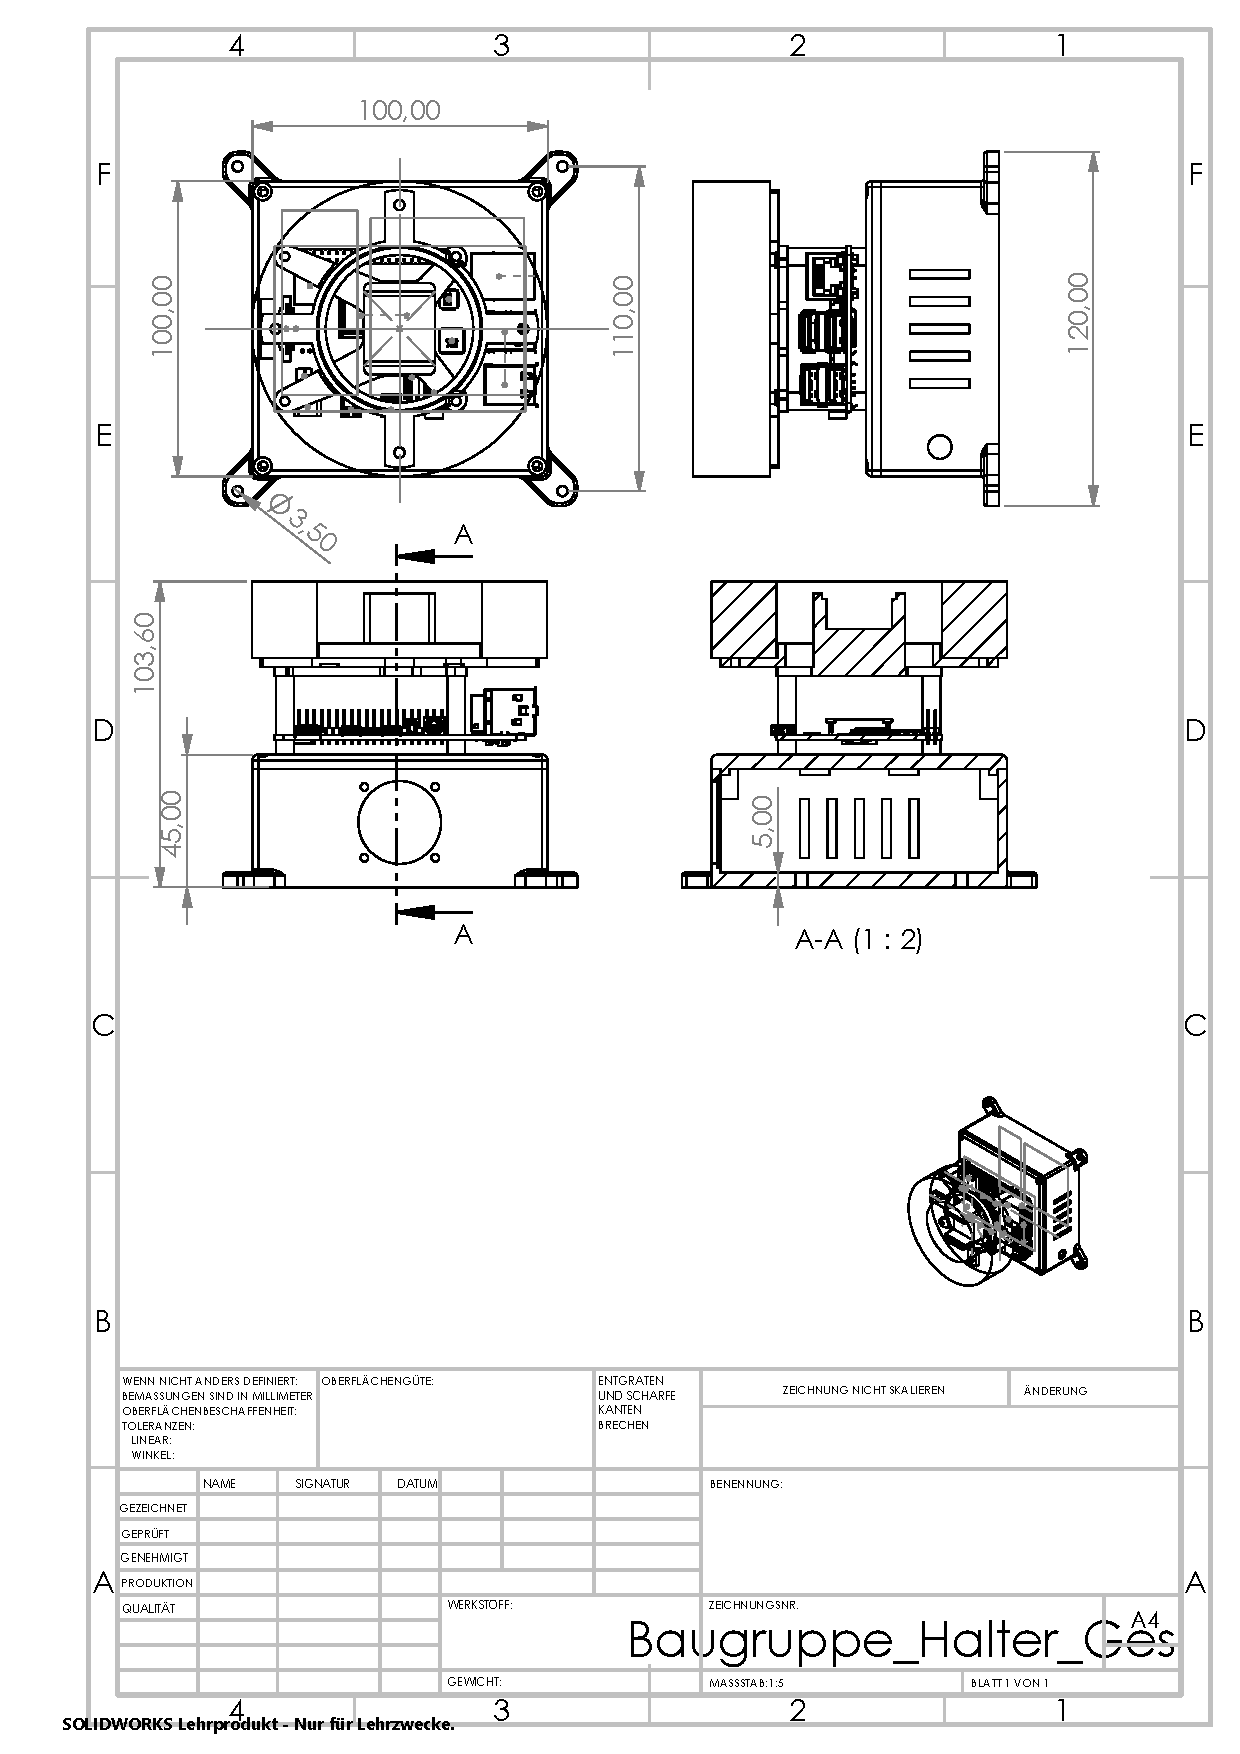
\includepdf[pages=-]{Baugruppe_Halter_Ges.pdf}

\chapter{Fotos Technikbox}
\label{app:fotos_technikbox}

\begin{figure}[h]
  \centering
  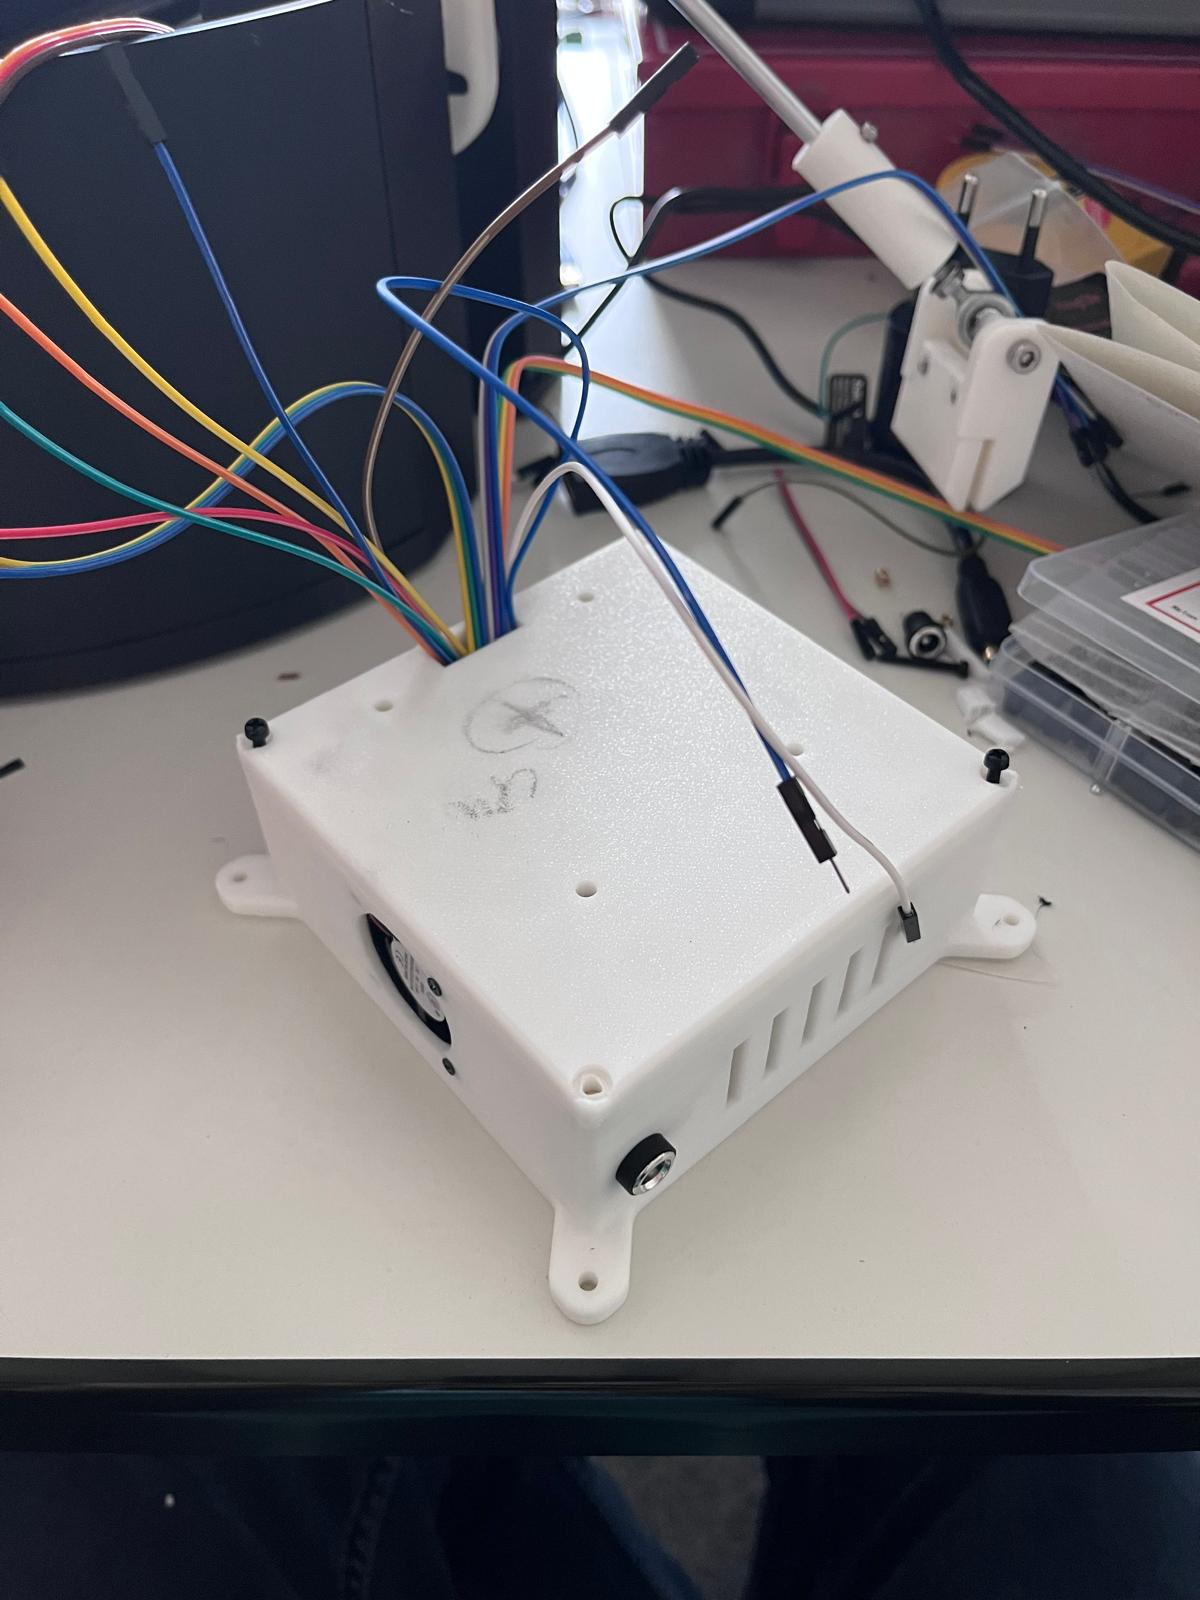
\includegraphics[width=0.7\textwidth]{E2.jpg}
  \caption{Technikbox geschlossen}
\end{figure}

\end{document}
